% Official VLDB 2027 / PVLDB Volume 20 template, based on acmart v2.19.
\documentclass[sigconf,nonacm]{acmart}

%%% do not modify the following VLDB block %%%
%%% VLDB block start %%%
\usepackage{pvldb}
%%% VLDB block end %%%

% DOI and pages are assigned at camera-ready time.
\renewcommand\vldbdoi{XX.XX/XXX.XX}
\renewcommand\vldbpages{XXX-XXX}
\renewcommand\vldbavailabilityurl{https://github.com/yanchaomei/SlabWalk-artifact}

\usepackage{booktabs}
\usepackage{graphicx}
\usepackage{array}
\usepackage{amsmath}
\usepackage{placeins}
\hypersetup{pdfauthor={Chaomei Yan}}

\newcommand{\sys}{SlabWalk}
\newcommand{\uppergraph}{resident upper graph}
\newcommand{\xblock}{Slab}
\newcommand{\xblocks}{Slabs}
\newcommand{\cn}{CN}
\newcommand{\mn}{MN}
\newcommand{\ef}{\texttt{ef}}
\newcolumntype{L}[1]{>{\raggedright\arraybackslash}p{#1}}

% Headline and resource claims are generated only after the final evidence gate passes.
% Generated from gated manuscript_claims.json. Do not edit.
% gate-sha256: fea1f82f79120a94c7327a1e3009a4b3163b00a8e4c8ae0e3a0a926e04fdfbdd
% claims-sha256: 8297ca77006fcab836ed0d0f0c351127f7dac768804fd68fd597275e66bfe17b
\newcommand{\ClaimGateSha}{fea1f82f79120a94c7327a1e3009a4b3163b00a8e4c8ae0e3a0a926e04fdfbdd}
\newcommand{\ClaimFrontierRecallFloor}{0.90}
\newcommand{\ClaimFrontierRecallTolerance}{0.002}
\newcommand{\ClaimFrontierQpsMin}{9.99}
\newcommand{\ClaimFrontierQpsMax}{13.46}
\newcommand{\ClaimFrontierPostsMin}{17.13}
\newcommand{\ClaimFrontierPostsMax}{27.22}
\newcommand{\ClaimDhnswDeepRecall}{0.923}
\newcommand{\ClaimDhnswSiftRecall}{0.905}
\newcommand{\ClaimDhnswTtiRecall}{0.601}
\newcommand{\ClaimCachePostReduction}{83.2}
\newcommand{\ClaimCacheQpsLoss}{23.2}
\newcommand{\ClaimProfileDistanceShare}{5.16}
\newcommand{\ClaimColocationQpsLoss}{64.5}
\newcommand{\ClaimColocationPostIncrease}{98.4}
\newcommand{\ClaimColocationByteIncrease}{54.9}
\newcommand{\ClaimColocationRecall}{0.98907}
\newcommand{\ClaimResidentNodes}{62,529}
\newcommand{\ClaimResidentBytesMB}{32.0}
\newcommand{\ClaimResidentQpsGain}{31.1}
\newcommand{\ClaimResidentRemotePosts}{122.3}
\newcommand{\ClaimBudgetFiveGiB}{0.46}
\newcommand{\ClaimBudgetFullGiB}{2.78}
\newcommand{\ClaimWorkerOneKqps}{1.24}
\newcommand{\ClaimWorkerFortyKqps}{14.74}
\newcommand{\ClaimWorkerGain}{11.9}
\newcommand{\ClaimWorkerRecall}{0.989}
\newcommand{\ClaimLegacyAmplification}{11.24}
\newcommand{\ClaimFixedAmplification}{3.05}
\newcommand{\ClaimVariableAmplification}{1.63}
\newcommand{\ClaimVariableSidecarGiB}{2.42}
\newcommand{\ClaimVariableCnRssGiB}{8.54}
\newcommand{\ClaimVariableOneMnQps}{2960.4}
\newcommand{\ClaimVariableFiveMnQps}{2969.4}
\newcommand{\ClaimVariableOneMnRssGiB}{10.01}
\newcommand{\ClaimVariableFiveMnRssGiB}{5.51}
\newcommand{\ClaimVariableReadGini}{0.0048}
\newcommand{\ClaimRdmaPayloadSmallMeanUs}{4.24}
\newcommand{\ClaimRdmaPayloadLargeMeanUs}{5.57}
\newcommand{\ClaimRdmaPayloadSmallTailUs}{4.41}
\newcommand{\ClaimRdmaPayloadLargeTailUs}{5.78}
\newcommand{\ClaimRdmaPayloadMeanSpan}{1.31}
\newcommand{\ClaimRdmaPayloadTailSpan}{1.31}
\newcommand{\ClaimRdmaQpOneMops}{3.83}
\newcommand{\ClaimRdmaQpTwoMops}{7.21}
\newcommand{\ClaimRdmaMtuMeanSpan}{1.01}
\newcommand{\ClaimRdmaNumaDiffPct}{0.09}
\newcommand{\ClaimRdmaOutsOneMops}{0.26}
\newcommand{\ClaimRdmaOutsSixteenMops}{3.86}
\newcommand{\ClaimCoroOneKqps}{6.72}
\newcommand{\ClaimCoroFourKqps}{17.87}
\newcommand{\ClaimCoroFourTailMs}{2.70}
\newcommand{\ClaimCoroSixteenTailMs}{13.20}
\newcommand{\ClaimCoroFourToSixteenGainPct}{3.0}
\newcommand{\ClaimTopKQpsSpanPct}{1.9}
\newcommand{\ClaimZipfQpsDiffPct}{1.3}
\newcommand{\ClaimZipfTailDiffPct}{0.3}
\newcommand{\ClaimTopologyRecall}{0.909}
\newcommand{\ClaimTopologyLoopbackKqps}{4.19}
\newcommand{\ClaimTopologyRemoteKqps}{0.294}
\newcommand{\ClaimTopologyLoopbackLatencyMs}{2.20}
\newcommand{\ClaimTopologyRemoteLatencyMs}{18.46}
\newcommand{\ClaimTopologyRemoteNetworkMs}{17.94}
\newcommand{\ClaimRefreshMinRecords}{6.4}
\newcommand{\ClaimRefreshMaxRecords}{12.4}
\newcommand{\ClaimRefreshRecall}{0.97662}
\newcommand{\ClaimTtiSqEightRecall}{0.864}
\newcommand{\ClaimTtiRqTwoRecall}{0.815}
\newcommand{\ClaimTtiRqFourRecall}{0.862}
\newcommand{\ClaimTtiFpRecall}{0.961}
\newcommand{\ClaimTtiFpQps}{260}
\newcommand{\ClaimTtiFpPosts}{3,870}
\newcommand{\ClaimBuildOneMSiftSeconds}{20.62}
\newcommand{\ClaimBuildOneMSiftCiSeconds}{0.07}
\newcommand{\ClaimBuildOneMSiftRssGiB}{4.83}
\newcommand{\ClaimBuildOneMSiftRegionGiB}{4.30}
\newcommand{\ClaimBuildOneMDeepSeconds}{18.49}
\newcommand{\ClaimBuildOneMDeepCiSeconds}{0.05}
\newcommand{\ClaimBuildOneMDeepRssGiB}{4.71}
\newcommand{\ClaimBuildOneMDeepRegionGiB}{3.35}
\newcommand{\ClaimBuildOneMGistSeconds}{25.48}
\newcommand{\ClaimBuildOneMGistCiSeconds}{0.05}
\newcommand{\ClaimBuildOneMGistRssGiB}{8.51}
\newcommand{\ClaimBuildOneMGistRegionGiB}{7.88}
\newcommand{\ClaimBuildTenMDeepSeconds}{278.4}
\newcommand{\ClaimBuildTenMDeepCiSeconds}{4.9}
\newcommand{\ClaimBuildTenMDeepResidentSeconds}{2.16}
\newcommand{\ClaimBuildTenMDeepGiB}{35.3}
\newcommand{\ClaimBuildTenMSiftSeconds}{247.2}
\newcommand{\ClaimBuildTenMSiftCiSeconds}{0.5}
\newcommand{\ClaimBuildTenMSiftResidentSeconds}{3.63}
\newcommand{\ClaimBuildTenMSiftGiB}{28.9}
\newcommand{\ClaimBuildTenMTtiSeconds}{290.1}
\newcommand{\ClaimBuildTenMTtiCiSeconds}{1.0}
\newcommand{\ClaimBuildTenMTtiResidentSeconds}{4.27}
\newcommand{\ClaimBuildTenMTtiGiB}{39.2}


\begin{document}
\raggedbottom

\title[\sys: Expansion-Oriented Access Structure]{\sys: An Expansion-Oriented Physical Access Structure for Disaggregated Vector Search}

\author{Chaomei Yan}
\email{yanchaomei@mail.ustc.edu.cn}
\affiliation{%
  \institution{University of Science and Technology of China}
  \city{Hefei}
  \country{China}
}

\begin{abstract}
High-dimensional vector indexes often outgrow the DRAM of a serving compute
node.  Disaggregated memory decouples index capacity from compute, but an
in-memory HNSW layout is a poor remote layout: one level-0 expansion becomes a
neighbor-list read followed by many vector reads.  On our RoCE cluster, this
path exhausts the compute node's posted-operation rate before network
bandwidth.  The limiting choice is therefore the physical unit retrieved by
one remote access.

We present \sys{}, a physical access structure derived from an authoritative
HNSW index.  Each Slab stores the neighbor identifiers, scoring payloads, and
rerank addresses needed for one level-0 expansion, allowing one remote read to
supply one graph decision.  Resident upper navigation removes serial descent
reads, and budgeted physical design controls memory, transfer, and recall.  At
matched search width and high recall on repeated DEEP-10M and SIFT-10M
frontiers, \sys{} delivers \ClaimFrontierQpsMin--\ClaimFrontierQpsMax$\times$
the QPS of a same-binary SHINE-derived node/vector path while issuing
\ClaimFrontierPostsMin--\ClaimFrontierPostsMax$\times$ fewer posted reads.
Frontiers over seven 1M and three 10M workloads, together with controlled cost
and lifecycle experiments, show when expansion-oriented retrieval helps and
when representation quality or transfer becomes the next limit.
\end{abstract}

\maketitle

%%% do not modify the following VLDB block %%%
%%% VLDB block start %%%
\vldbtopmatter
%%% VLDB block end %%%

%================================================================
%================================================================
\section{Introduction}
\label{sec:intro}

Vector similarity search has become a serving primitive for vector
databases~\cite{milvus,manu,vbasesurvey}, recommender
systems~\cite{youtubednn,airbnb}, and retrieval-augmented
generation~\cite{rag,retro}.  HNSW~\cite{hnsw} leads the in-memory recall--throughput
frontier~\cite{nsg,wangsurvey}, but assumes that vectors and graph
records fit in local DRAM\@.  At billion-vector scale, raw fp32 payloads alone
occupy hundreds of gigabytes before graph edges and serving state; replicating
that index across serving nodes compounds the capacity cost~\cite{shine}.

Sharding vectors into independent graph indexes scales capacity, but excludes
cross-partition edges and requires probing multiple local indexes~\cite{shine,dhnsw}.
Disaggregated memory offers another physical design: passive
memory nodes hold registered index regions, while compute nodes execute the
walk.  It can preserve one authoritative HNSW graph, but only if the graph's
physical organization matches remote retrieval.

The physical retrieval unit need not match the in-memory node record.  Before
HNSW can choose its next candidate, it must read the current candidate's
neighbors, score them, and update the beam.  A node/vector layout realizes this
single decision as one list retrieval followed by as many as $d(u)$ vector
retrievals.  A routed-partition layout moves a larger subgraph and searches it
locally.  SlabWalk materializes the expansion itself, the smallest physical
object that contains every dependency of the next graph decision.  RDMA is the
transport used in our implementation; aligning storage with graph execution is
the access-method contribution.

\begin{figure*}[t]
\centering
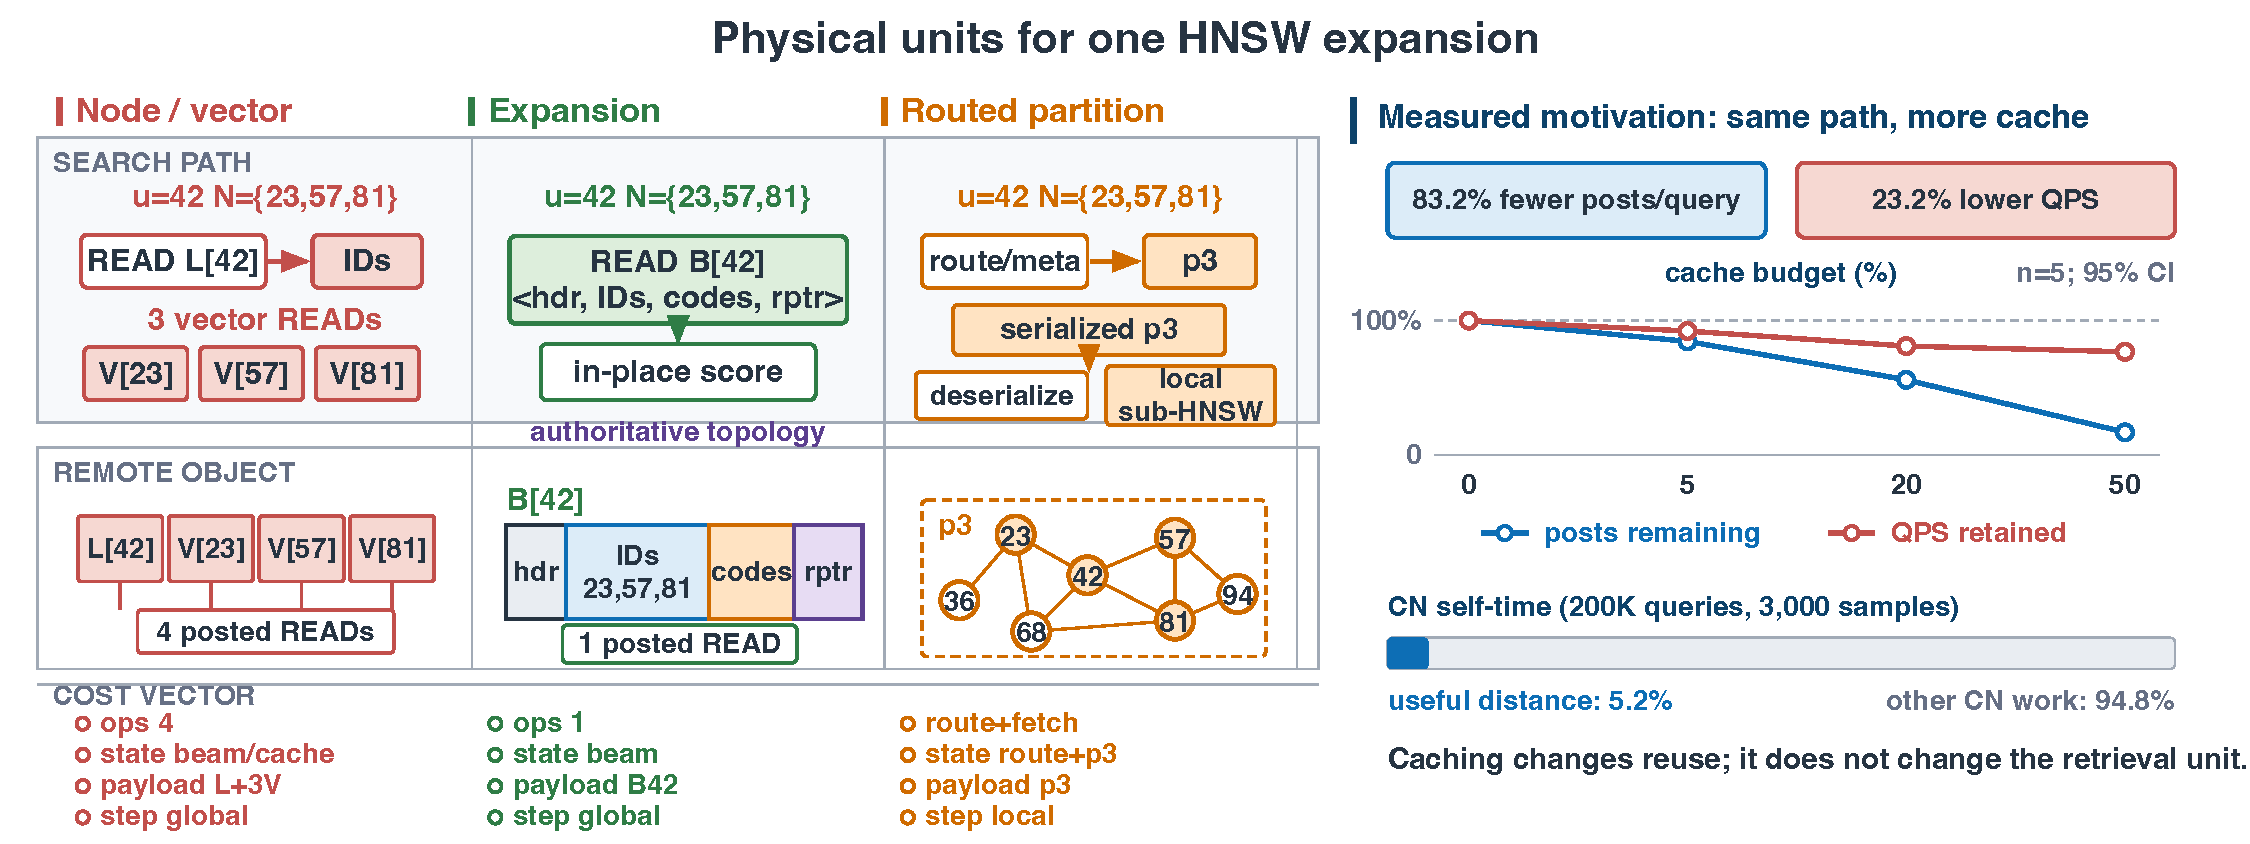
\includegraphics[width=0.88\textwidth]{figs/fig_physical_units.pdf}
\caption{Physical design space for one HNSW expansion.  The left matrix aligns
the retrieval path, stored object, and cost vector of node/vector, expansion,
and routed-partition organizations.  The SIFT-1M control on the right sweeps a
same-path CN cache and profiles query-only CN work; points are five-run means
with 95\% Student-$t$ intervals.}
\Description{A matrix compares the retrieval path, stored bytes, and cost of
node/vector records, one contiguous expansion record, and a routed serialized
partition.  A measured SIFT-1M inset plots normalized posts and QPS at four
cache budgets and separates distance computation from other compute-node
work.}
\label{fig:physical-units}
\end{figure*}

SHINE and d-HNSW occupy the neighboring points in
Figure~\ref{fig:physical-units}.  SHINE preserves a global HNSW and reduces
remote traffic with caching, segmentation, and routing, while retaining
node/vector retrieval~\cite{shine}.  d-HNSW routes through a meta-HNSW.  It
fetches and deserializes selected sub-HNSW partitions before local
search~\cite{dhnsw}.  Caching changes reuse but retains fine-grained retrieval;
partition fetching changes the search and ownership model.  SlabWalk instead
changes the retrieval unit while retaining the global walk.

On our 100\,Gbps RoCE cluster, the node/vector path reaches a compute-side
posted-operation ceiling before saturating the link or memory node.
Figure~\ref{fig:physical-units} tests a same-path cache remedy with a
fixed query pool: a cache sweep measures both posts and QPS, while a
query-only \texttt{perf} profile measures the fraction of CN self time spent in
distance arithmetic.  At a 50\% cache budget, the path issues
\ClaimCachePostReduction\% fewer posts yet delivers \ClaimCacheQpsLoss\%
lower QPS; useful distance arithmetic accounts for only
\ClaimProfileDistanceShare\%
of sampled CN self time.  The cache removes remote reads, but its probes,
eviction, and bookkeeping remain on the per-node path; fewer remote objects do
not produce higher throughput in this control.

We present \sys{}, which derives an expansion-oriented physical access
structure from an authoritative HNSW index.  Each Slab record contains the neighbor identifiers, compact scoring
codes, and exact-rerank addresses required by one level-0 expansion.  A
matching query strategy descends an exact resident upper graph, reads one Slab
record for each remote expansion, scores its live neighbors in place, and
reranks the surviving candidates with authoritative fp32 vectors.  Degree-bounded
materialization, variable records, code selection, and block-cyclic placement
keep the derived structure within memory, recall, and link budgets.

The scope is a read-mostly access structure over an already built HNSW graph.
Memory nodes remain passive, and the authoritative graph remains the source
for cold fallback, exact reranking, and rebuild.  Seven repeated 1M frontiers
test workload breadth, while repeated DEEP-10M, SIFT-10M, and TTI-10M
frontiers test scale.  Separate controls isolate access cost, concurrency,
placement, construction, and lifecycle behavior.
Transactional online mutation, automatic reconfiguration, and billion-scale
initial construction are outside this paper's scope.

We make three technical contributions:
\begin{itemize}
  \item \textbf{Expansion-oriented access abstraction.}  We identify access
  amplification in passive-RDMA HNSW and make one dependency-complete expansion
  the remote access unit.  A Slab record preserves graph topology and
  authoritative ownership while paying one retrieval per materialized
  expansion.
  \item \textbf{Expansion-aligned query operator.}  An exact resident upper
  graph removes serial descent reads, compact in-place scoring advances the
  global beam, and bounded reranking re-scores surviving candidates in fp32.
  The operator retains authoritative fallback for unmaterialized records.
  \item \textbf{Budgeted, self-describing physical design.}  Partial materialization,
  variable packed records, code guards, and block-cyclic placement bound CN
  state, MN storage, transfer, and representation error.  An offline advisor
  rejects infeasible measured layouts and selects by the lower 95\% confidence
  bound on QPS.  Construction derives Slabs and resident navigation from one
  validated snapshot; a verified descriptor records the selected format and
  placement.  Rematerialization is explicitly offline.
\end{itemize}
At matched high recall on DEEP-10M and SIFT-10M, the integrated path delivers
\ClaimFrontierQpsMin--\ClaimFrontierQpsMax$\times$ the QPS of same-binary
node/vector access while issuing \ClaimFrontierPostsMin--\ClaimFrontierPostsMax$\times$
fewer posted reads.  Three-system frontiers cover seven 1M workloads and three
10M workloads; mechanism controls connect the result to access, transfer,
storage, CN state, construction, and representation costs.

%================================================================
\section{Background and Motivation}
\label{sec:diagnosis}

\subsection{HNSW Expansion Semantics}
\label{sec:bg-ann}

Given a query $q\in\mathbb{R}^d$, approximate $k$-nearest-neighbor search
returns a set whose quality is measured by Recall@$k$.  HNSW first performs a
greedy descent through sparse upper layers, then searches the dense level-0
graph with a candidate beam~\cite{hnsw}.  To \emph{expand} candidate $u$, the
query processor reads $u$'s neighbor identifiers, scores each unvisited
neighbor against $q$, and updates the beam.  The next candidate depends on
these scores.  An expansion is therefore the dependency boundary at which the
walk can make its next graph decision, even though an in-memory implementation
may store the required inputs in several records.

Disaggregation makes this distinction visible.  A compute node (CN) issues
one-sided reads and performs every graph and distance operation; a memory node
(MN) only exposes registered bytes.  The graph algorithm does not dictate
that a remote record must equal an in-memory C++ object.  Physical organization
decides how many remote accesses and transferred bytes realize each logical
expansion.

\subsection{Physical Organizations for Remote HNSW}
\label{sec:opwall}

Table~\ref{tab:remote-objects} compares three physical organizations.  A
node/vector design uses the authoritative in-memory schema and pays per object.
An expansion design materializes one graph decision while retaining the global
graph.  A routed-partition design selects and transfers a subgraph, then
searches it locally.  Systems may combine these units with caching, routing, or
coalescing.

\begin{table*}[t]
\centering\scriptsize
\caption{Remote-HNSW physical organizations.  The node/vector row is
SHINE-derived, not an official reproduction.}
\label{tab:remote-objects}
\setlength{\tabcolsep}{2.6pt}
\begin{tabular}{L{0.14\textwidth}L{0.18\textwidth}L{0.20\textwidth}L{0.20\textwidth}L{0.20\textwidth}}
\toprule
Physical unit & Graph semantics & Work per retrieval & CN execution / state & Principal boundary \\
\midrule
Node / vector & One global HNSW & One list or one scoring vector &
Per-object lookup and beam scoring; cache plus query state &
$1+m_A(q,u)\leq 1+d(u)$ accesses per expansion; cache-path overhead \\
Expansion (SlabWalk) & One global HNSW & IDs, codes, and rerank addresses for
one expansion & Exact resident descent, in-place scoring, and bounded fp32 rerank &
Derived-structure bytes and compact-code error \\
Routed partition (d-HNSW) & Meta-HNSW plus selected sub-HNSW & Serialized
subgraph and vectors & Meta-index routing, partition state, deserialization, and local search &
Coverage, payload, deserialization, and rebuild \\
\bottomrule
\end{tabular}
\end{table*}

The choice is not ``small versus large reads'' in isolation.  A useful remote
unit must return enough work to advance the algorithm, preserve the desired
graph topology, and fit storage and transfer budgets.  SlabWalk chooses the
smallest dependency-complete unit that supplies the deployed walk with all inputs
for its next level-0 expansion.  Compact scoring can change candidate order,
but the edges and fp32 rerank targets remain those of the authoritative HNSW.

\subsection{Physical Cost Model and Design Requirements}
\label{sec:operation-model}

For access method $A$ and query $q$, let $\mathcal{E}_A(q)$ be the sequence of
remote level-0 expansions, $D_A(q)$ the upper-descent reads, $c_A(q,u)$ the
reads needed to realize expansion $u$, and $R_A(q)$ the exact rerank reads.  The
logical remote-access cost is
\begin{equation}
  \Omega_A(q)=D_A(q)+\sum_{u\in\mathcal{E}_A(q)}c_A(q,u)+R_A(q).
  \label{eq:logical-cost}
\end{equation}
For node/vector storage, let $m_A(q,u)\leq d(u)$ be the number of neighbor
payloads that require distinct remote retrievals after visited and cache checks.
Then $c_A(q,u)=1+m_A(q,u)$.  After one CN-local address lookup, a materialized
Slab has $c_A(q,u)=1$.  A routed partition changes the operator sequence: it
amortizes one fetch over local subgraph expansions but adds meta-index routing,
partition transfer, deserialization, and local search.

We characterize each organization by the physical-cost vector
\begin{equation}
  \mathcal{K}_A(q)=\langle\Omega_A(q),\mathcal{B}_A(q),U_A(q),\mathcal{S}_A\rangle,
  \label{eq:physical-cost-vector}
\end{equation}
where $\mathcal{B}_A(q)$ is transferred bytes, $U_A(q)$ is CN search work apart
from remote-operation service, and $\mathcal{S}_A$ is persistent CN state.
\emph{Access amplification} is $\Omega_A(q)/|\mathcal{E}_A(q)|$; we also report
raw posted reads/query.  \emph{Storage amplification} is total MN index bytes,
including the authoritative HNSW and derived state, divided by authoritative
HNSW bytes.  Reporting all four components is necessary because a larger
retrieval can reduce $\Omega$ while increasing bytes, CN work, or state.

For our passive-RDMA implementation, the issuing-side component admits the
first-order accounting relation
\begin{equation}
  T_A(q)\approx U_A(q)+\tau\Omega_A(q),
  \label{eq:rdma-cost}
\end{equation}
where $\tau$ is amortized issuing-thread service demand per posted read.  It is
not raw network latency: outstanding reads overlap link delay, while the CN
still posts requests and processes completions.  Section~\ref{sec:eval-scaling}
varies payload, queue organization, outstanding depth, MTU, and NUMA placement
below the ANN stack.  These controls test the per-operation premise for this
implementation; we do not fit one shared $\tau$ to predict all three systems,
whose $U_A$, $\mathcal{B}_A$, and $\mathcal{S}_A$ differ.

Four requirements follow from the cost vector.  A remote record must contain
the dependency-complete inputs of an expansion; upper descent must not restore
a serial-read term; materialization and representation must fit MN, link, and
recall budgets; and intact records must be placeable across passive MNs without
a router.  Sections~\ref{sec:design}--\ref{sec:deployment} implement these
requirements; Section~\ref{sec:eval} measures each resource term.

%================================================================
\section{Physical Design Overview}
\label{sec:overview}

Request issue and completion processing consume CN resources in prior RDMA
systems~\cite{herd,fasst,erpc}; Section~\ref{sec:operation-model} measures the
same cost on our passive-READ path.  SlabWalk uses the paid remote operation to
return one useful graph step, namely an expansion.  Disk-resident graph indexes
make an analogous physical-design choice for pages and device parallelism,
where the expensive unit is different~\cite{starling,ssdpgvector}.

\subsection{Resource Constraints and Design Rules}
\label{sec:cost-model}

Each mechanism removes or bounds one measured cost.  Slab records remove
repeated retrievals within an expansion, and an exact resident upper graph
removes remote descent.  Degree budgets, compact codes, and variable records
limit storage; block-cyclic ownership distributes intact records; bounded fp32
reranking contains representation error.  We choose the access unit first,
then bound the resources that it consumes.

Let $f$ be the materialized node fraction, $b$ the scoring-code choice, $S$
the MN stripe count, and $R$ the rerank bound.  A deployment selects them under
explicit constraints.  Here, $\Theta_{\mathrm{CN}}$ is the measured
compute-side posted-operation capacity,
\begin{align}
  \mathcal{M}_{\mathrm{Slab}}(f,b) &\leq M_{\mathrm{MN}}, &
  \mathcal{M}_{\mathrm{resident}} &\leq M_{\mathrm{CN}}, \\
  \mathrm{QPS}\cdot\overline{\Omega}(f,b,R,\ef) &\leq \Theta_{\mathrm{CN}}, &
  \mathrm{QPS}\cdot\overline{\mathcal{B}}(f,b,S) &\leq B_{\mathrm{link}}, \\
  \mathrm{QPS}\cdot\overline{U}(f,b,R,\ef) &\leq C_{\mathrm{CN}}, &
  \mathrm{Recall}(f,b,R,\ef) &\geq \mathrm{Recall}_{\mathrm{target}}.
  \label{eq:deployment-constraints}
\end{align}
These constraints define an offline selection problem over measured candidates.
The advisor rejects layouts that exceed a resource or recall target, then
maximizes the lower endpoint of a two-sided Student-$t$ 95\% QPS interval; mean
QPS and a stable identifier break ties.  It does not extrapolate to unmeasured
layouts or reconfigure a running index.  Section~\ref{sec:eval-index-cost}
tests the rule with a held-out split.

\subsection{Build and Query Workflow}
\label{sec:design-overview}

\begin{figure*}[t]
\centering
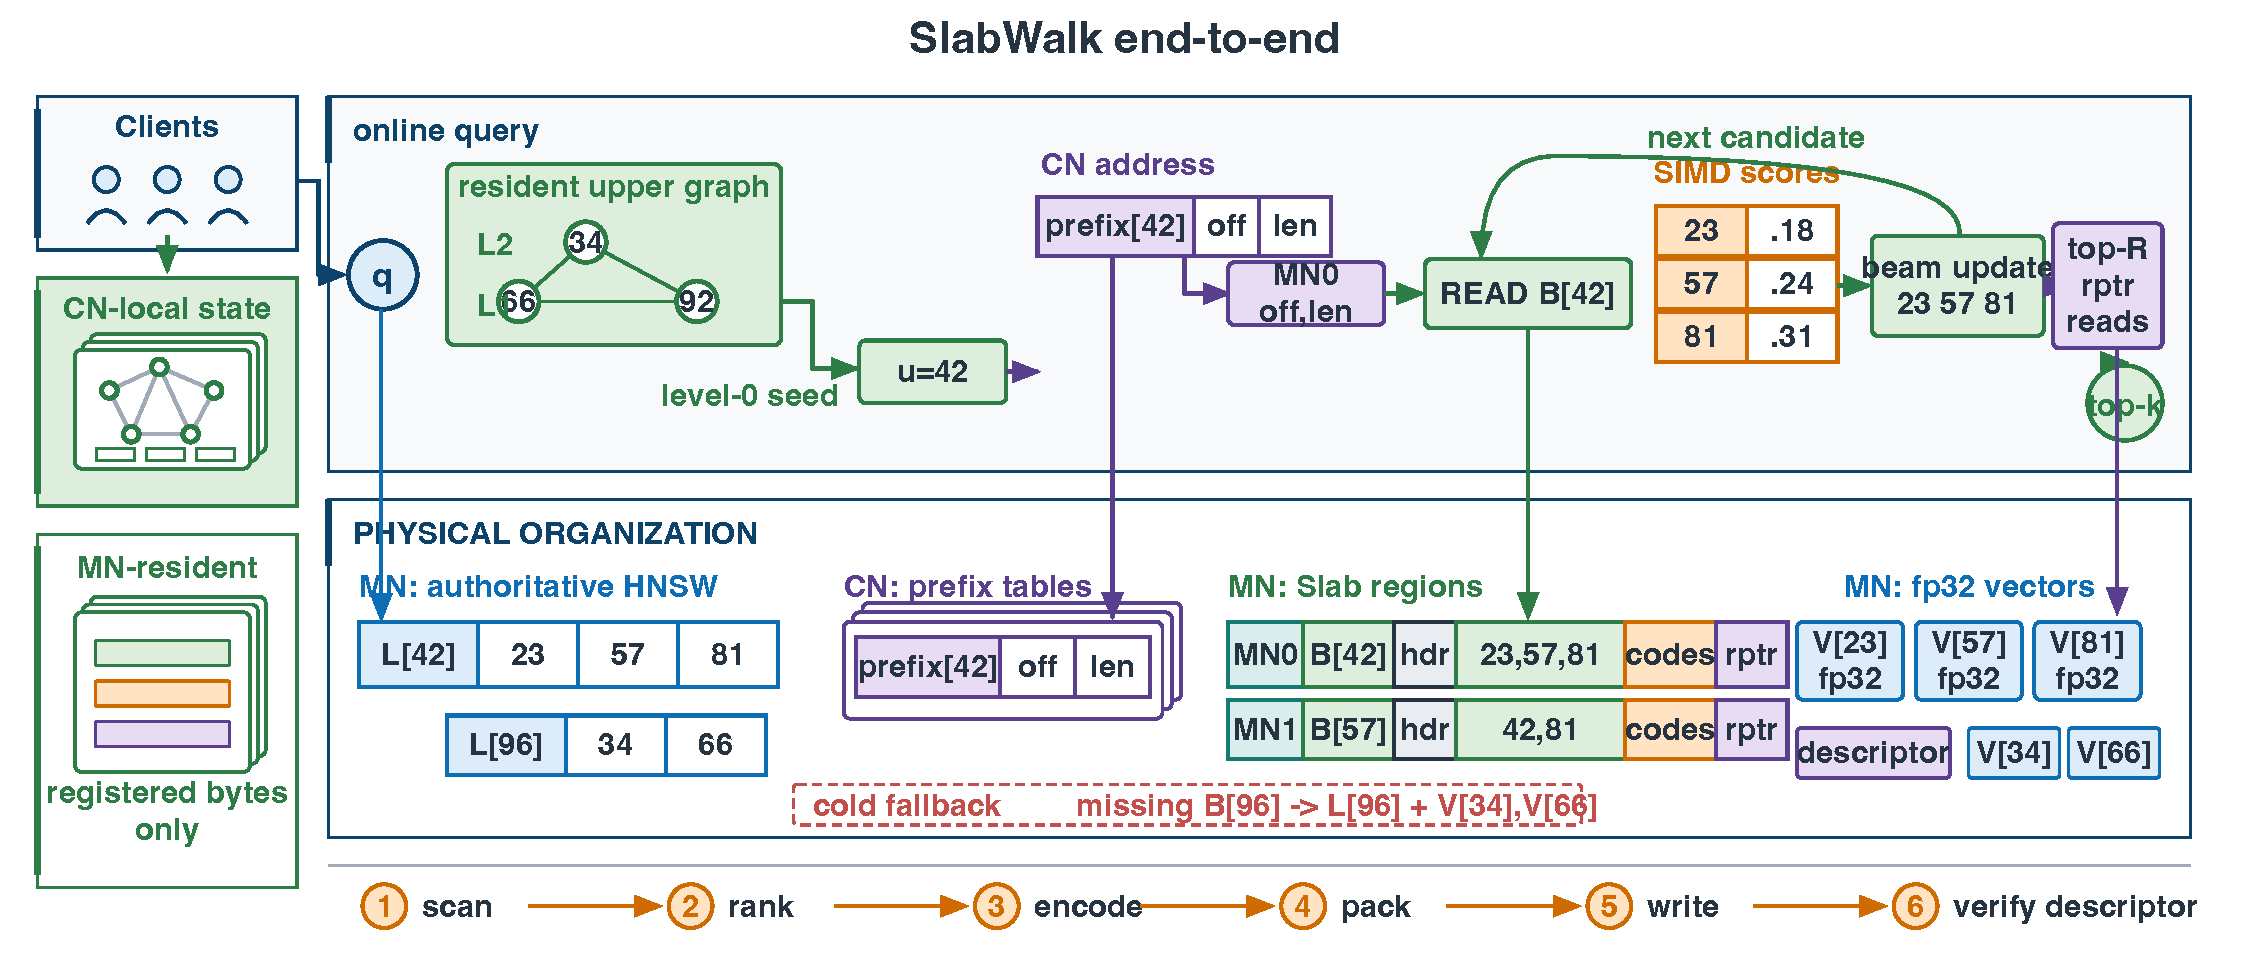
\includegraphics[width=0.86\textwidth]{figs/overview.pdf}
\caption{SlabWalk workflow.  The upper lane follows one query from resident
descent through a Slab read, beam update, and fp32 rerank.  The aligned lower
lane identifies the authoritative HNSW, CN address metadata, Slab regions, and
fp32 vectors touched by those operations.  The footer shows offline derivation.}
\Description{Aligned search and physical-layout lanes map resident descent,
one-read expansion, fallback, and reranking to authoritative HNSW records,
prefix tables, Slab regions, and fp32 vectors.  A short footer shows the six
offline derivation stages.}
\label{fig:overview}
\end{figure*}

Figure~\ref{fig:overview} aligns online operations with their physical records.
CNs execute the graph walk; passive MNs expose registered HNSW, Slab, and fp32
regions.  During build, an initiating CN records level-0 offsets and
in-degrees, chooses a materialization set under the degree budget, and encodes
and packs records from the unchanged HNSW\@.  In the
full fixed-record path, pinned workers fill bounded contiguous staging windows,
and each complete window is published to its owning MN region with one RDMA
WRITE.  The builder then writes and
verifies a self-describing layout descriptor.  Serving CNs copy the exact upper
graph at startup; the initiating CN reuses both the authoritative snapshot and,
for RaBitQ, the deterministic rotation already produced by the Slab builder.
Online, a CN reaches the same level-0 seed and
scores the ordinary global beam from $B[u]$.  It sends cold candidates to the
authoritative path and exactly reranks the top-$R$ through fp32 addresses; MNs
neither parse graphs nor execute routing or distance kernels.

\subsection{Ownership and Invariants}

SlabWalk preserves two invariants.  \emph{Authoritative ownership} means the
HNSW remains the sole source of truth for topology and fp32 vectors.  A Slab is
a materialized access record: it copies edge identities and scoring payloads
but does not acquire independent graph ownership.  Compact scoring may change
the visited sequence.  \emph{Controlled fallback} means an unmaterialized
record returns to the authoritative node/vector path without changing the
query's graph state.  Compact codes are intentionally different: they may
perturb candidate order before exact reranking, so we report their recall
boundary rather than call the path byte-identical.

Construction derives Slabs and the resident upper graph from the same
validated authoritative snapshot.  The descriptor records format, code,
ownership, and per-MN extents and is verified before Slab reads are enabled.
The current system does not switch versions while serving; offline refresh
therefore cannot expose a query to mixed derived versions.

Throughout the paper, \sys{} denotes the derived physical access structure:
Slab records, CN-local address metadata, resident upper navigation, and the
matching query path.  It is neither the authoritative HNSW nor a query-result
cache.  This terminology keeps the storage owner, derived layout, and access
operator distinct.

%================================================================
\section{Expansion-Oriented Data Layout}
\label{sec:design}

\subsection{Slab Record Layout}
\label{sec:layout}

\begin{figure*}[t]
\centering
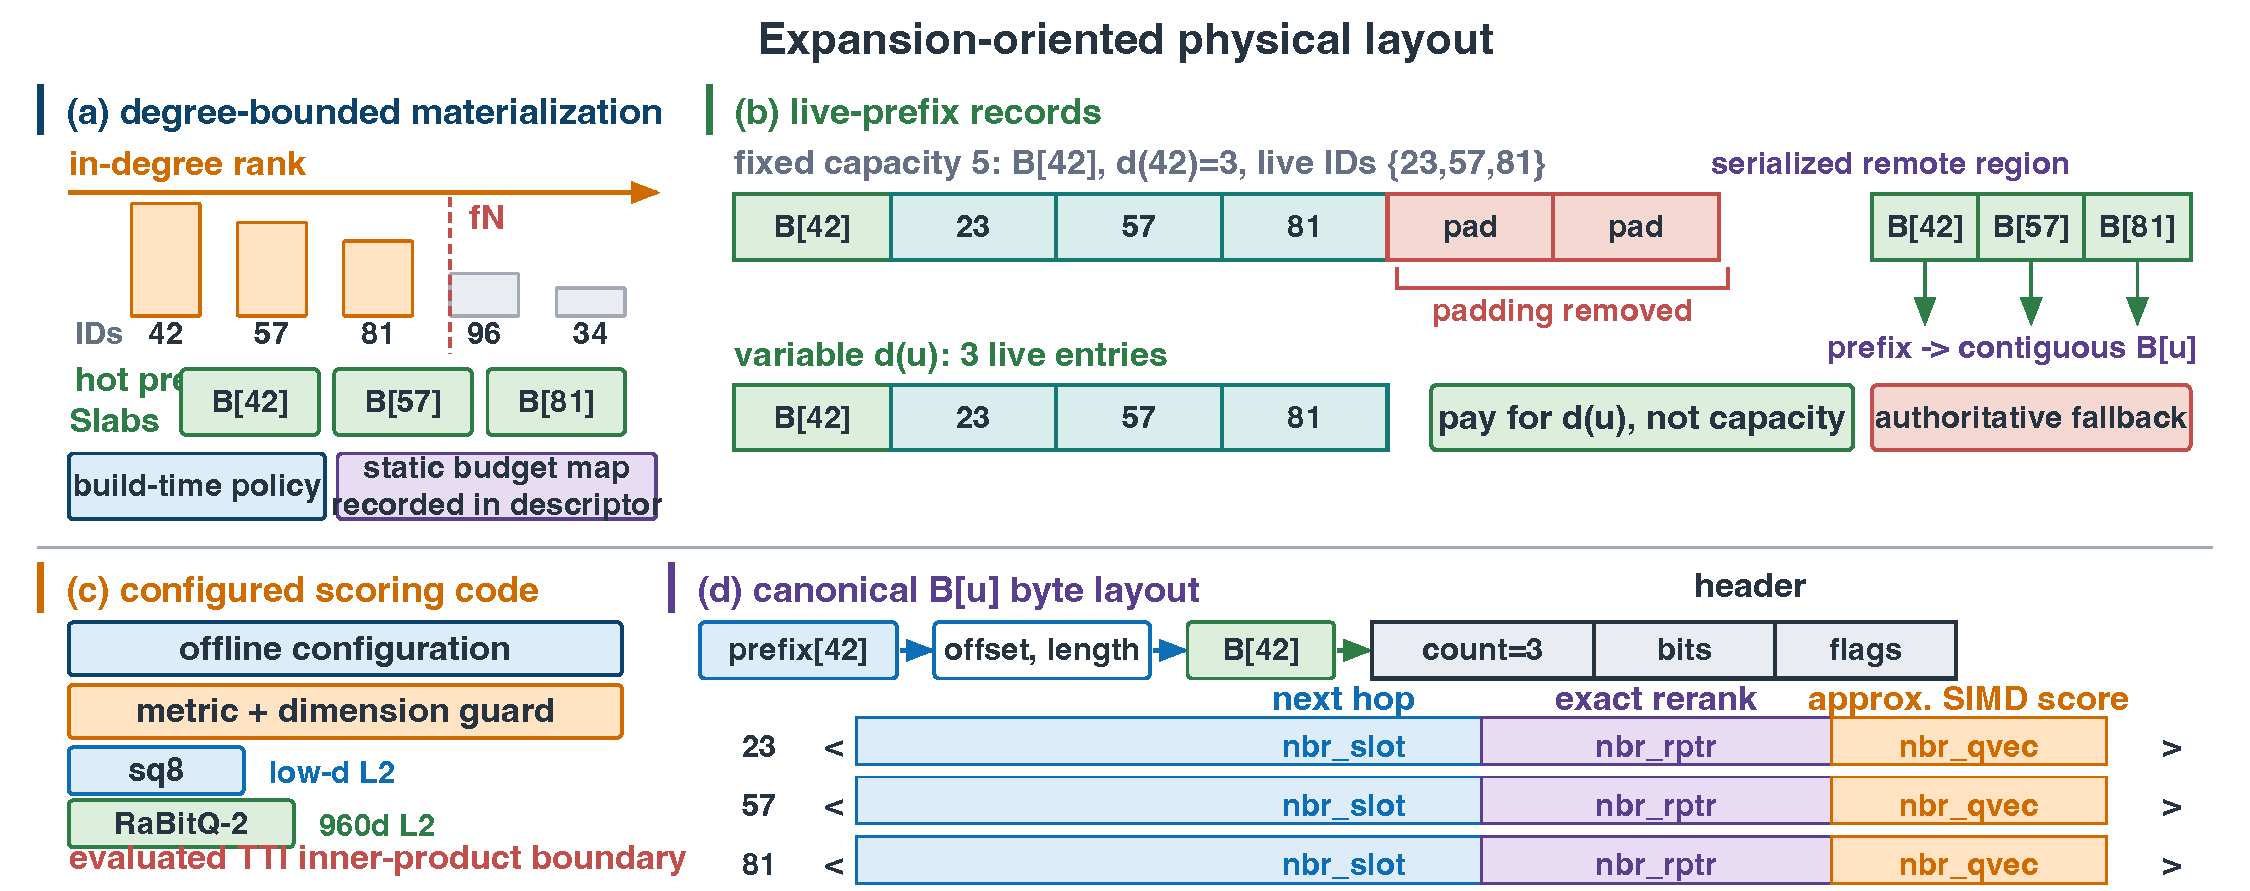
\includegraphics[width=0.86\textwidth]{figs/fig_slab_layout.pdf}
\caption{Expansion-oriented layout: (a) degree-bounded selection, (b)
live-prefix records, (c) guarded scoring codes, and (d) byte-level record
resolution.  \texttt{nbr\_slot} drives traversal, \texttt{nbr\_qvec} supports
beam scoring, and \texttt{nbr\_rptr} addresses authoritative fp32 vectors.}
\Description{A rank cut selects the materialized prefix, a serialized region
contrasts fixed and live-prefix records, and a magnified Slab shows the header
and three neighbor tuples.  Compact qvec fields feed approximate beam scoring,
while rptr fields address authoritative fp32 vectors for exact rerank.}
\label{fig:slab-layout}
\end{figure*}

Figure~\ref{fig:slab-layout}(a--d) connects the deployment guards to the
byte-level record used by each expansion.  For dense slot $u$, SlabWalk stores
\begin{equation}
  B[u]=\left\langle\texttt{header},
  {\bigl(\texttt{nbr\_slot}_{i},\texttt{nbr\_rptr}_{i},
  \texttt{nbr\_qvec}_{i}\bigr)}_{i=1}^{d(u)}
  \right\rangle.
  \label{eq:slab-record}
\end{equation}
The header stores the live count and code configuration.  Every live neighbor
carries a \texttt{nbr\_slot} for the next Slab without MN pointer chasing, a
\texttt{nbr\_qvec} for in-place approximate scoring, and a
\texttt{nbr\_rptr} for authoritative fp32 rerank.  Partially co-locating these
payloads would force a second read before scoring uncovered neighbors.

\begin{table*}[t]
\centering\small
\caption{Byte-level Slab record.  $Q(d,b)$ is $d$ bytes for sq8,
$\lceil d/2\rceil$ for sq4, or an 8-byte norm/dot prefix plus a packed RaBitQ
code.  Variable records store only the live degree.}
\label{tab:slab-layout}
\setlength{\tabcolsep}{3pt}
\begin{tabular}{L{0.13\textwidth}L{0.19\textwidth}L{0.11\textwidth}L{0.27\textwidth}L{0.18\textwidth}}
\toprule
Scope & Field & Bytes & Query use & Replication \\
\midrule
Record & \texttt{count}, bits, flags & 8 & Bound live prefix and decode codes & Once per materialized node \\
Neighbor & \texttt{nbr\_slot} + padding & 8 & Dense next-hop address & Once per materialized edge \\
Neighbor & \texttt{nbr\_rptr} & 8 & Authoritative fp32 address & Once per materialized edge \\
Neighbor & \texttt{nbr\_qvec} & $Q(d,b)$ & In-place approximate scoring & Once per materialized edge \\
Record index & \texttt{prefix[slot]} & $8N+8S$ & Offset and length lookup & Once per CN \\
\bottomrule
\end{tabular}
\end{table*}

A \texttt{RemotePtr} carries MN id, byte offset, and length.  Variable layouts
use a CN-local prefix table.  Across $S$ MNs, each CN stores one
64-bit entry per graph slot plus one sentinel per MN, or $8(N+S)$ bytes.
Partial materialization additionally uses a $4N$-byte dense budget map.  Fully
materialized fixed records omit both structures.  The required metadata is loaded once at startup and
replicated per CN, so the query performs one local address lookup before its
one remote Slab read.  The MN parses nothing, and consecutive graph slots need
not be visited together.

\subsection{Degree-Bounded Materialization}
\label{sec:budget}

Full denormalization materializes one Slab per node and repeats a vector code
across incoming edges, multiplying the derived bytes.  Query traffic, however,
is heavy-tailed.  Build-time in-degree provides a query-independent hub proxy.
SlabWalk ranks nodes by that proxy, materializes the top-$fN$, and serves the
cold tail through the authoritative fp32 node/vector path.  This deterministic,
query-independent heuristic preserves the authoritative topology but makes no
optimality claim; compact scoring on materialized records may perturb beam
order before exact reranking.

Let $E_A(q)=|\mathcal{E}_A(q)|$.  Let $\mathcal{E}_{\mathrm{hot}}(q;f)$ and
$\mathcal{E}_{\mathrm{cold}}(q;f)$ partition these expansions under budget
$f$, with $\nu(q;f)=|\mathcal{E}_{\mathrm{hot}}|/E_A(q)$.  Ignoring upper
descent for the moment, its access cost is
\begin{equation}
  \Omega_A(q;f)=\nu(q;f)E_A(q)+
  \!\sum_{u\in\mathcal{E}_{\mathrm{cold}}(q;f)}
  \bigl(1+m_A(q,u)\bigr)+R_A(q).
  \label{eq:budget-access}
\end{equation}
For $W$ issuing workers and workload means $\overline{\Omega}(f)$ and
$\overline{\mathcal{B}}(f)$, the throughput envelope is
\begin{equation}
  \mathrm{QPS}_{\max}(f)\lesssim\min\left(
    \frac{W}{\overline{U}(f)+\tau\overline{\Omega}(f)},
    \frac{B_{\mathrm{link}}}{\overline{\mathcal{B}}(f)},
    \frac{C_{\mathrm{CN}}}{\overline{U}(f)}
  \right).
  \label{eq:budget-envelope}
\end{equation}
When the proxy captures hot hubs, early records reduce $\Omega(f)$ rapidly;
later records add bytes with diminishing access savings.  The measured
GIST-200K sweep tests this tradeoff directly: early materialization rapidly
reduces posts/query, while later records consume more bytes for diminishing
throughput gain.  The ranking proposes candidate points and the sweep selects
a feasible deployment point.  It is a build policy, not a runtime cache.

\subsection{Code and Record-Size Guards}

The materialization fraction bounds how many records are copied; the code
bounds bytes per copied edge.  We use scalar sq8 on the low-dimensional L2
frontiers and report recall at every operating point.  At 960 dimensions,
the full sq8 footprint exceeds the configured per-index region, while the
evaluated RaBitQ-2 layout~\cite{rabitq} fits.  Code choice is configured by
metric and dimension: we evaluate sq8 on the low-dimensional L2 datasets,
RaBitQ-2 on 960-dimensional GIST, and explicitly expose the scalar-code recall
boundary on inner-product TTI (Section~\ref{sec:eval-scope}).

Fixed records reserve $M_0^{\max}$ neighbor entries even when $d(u)$ is smaller,
wasting $M_0^{\max}-d(u)$ neighbor slots.  Variable records and the prefix table
fetch only the live payload; the repeated
GIST ledger in Section~\ref{sec:eval-index-cost} validates their physical byte
accounting and query behavior.  The epoch-tagged visited bitmap remains
query-local state and scales with graph size and coroutine count; it is
distinct from the replicated resident upper graph accounted separately in
Section~\ref{sec:eval-index-cost}.

%================================================================
\section{Search and Placement Strategy}
\label{sec:query-processing}

\begin{figure*}[t]
\centering
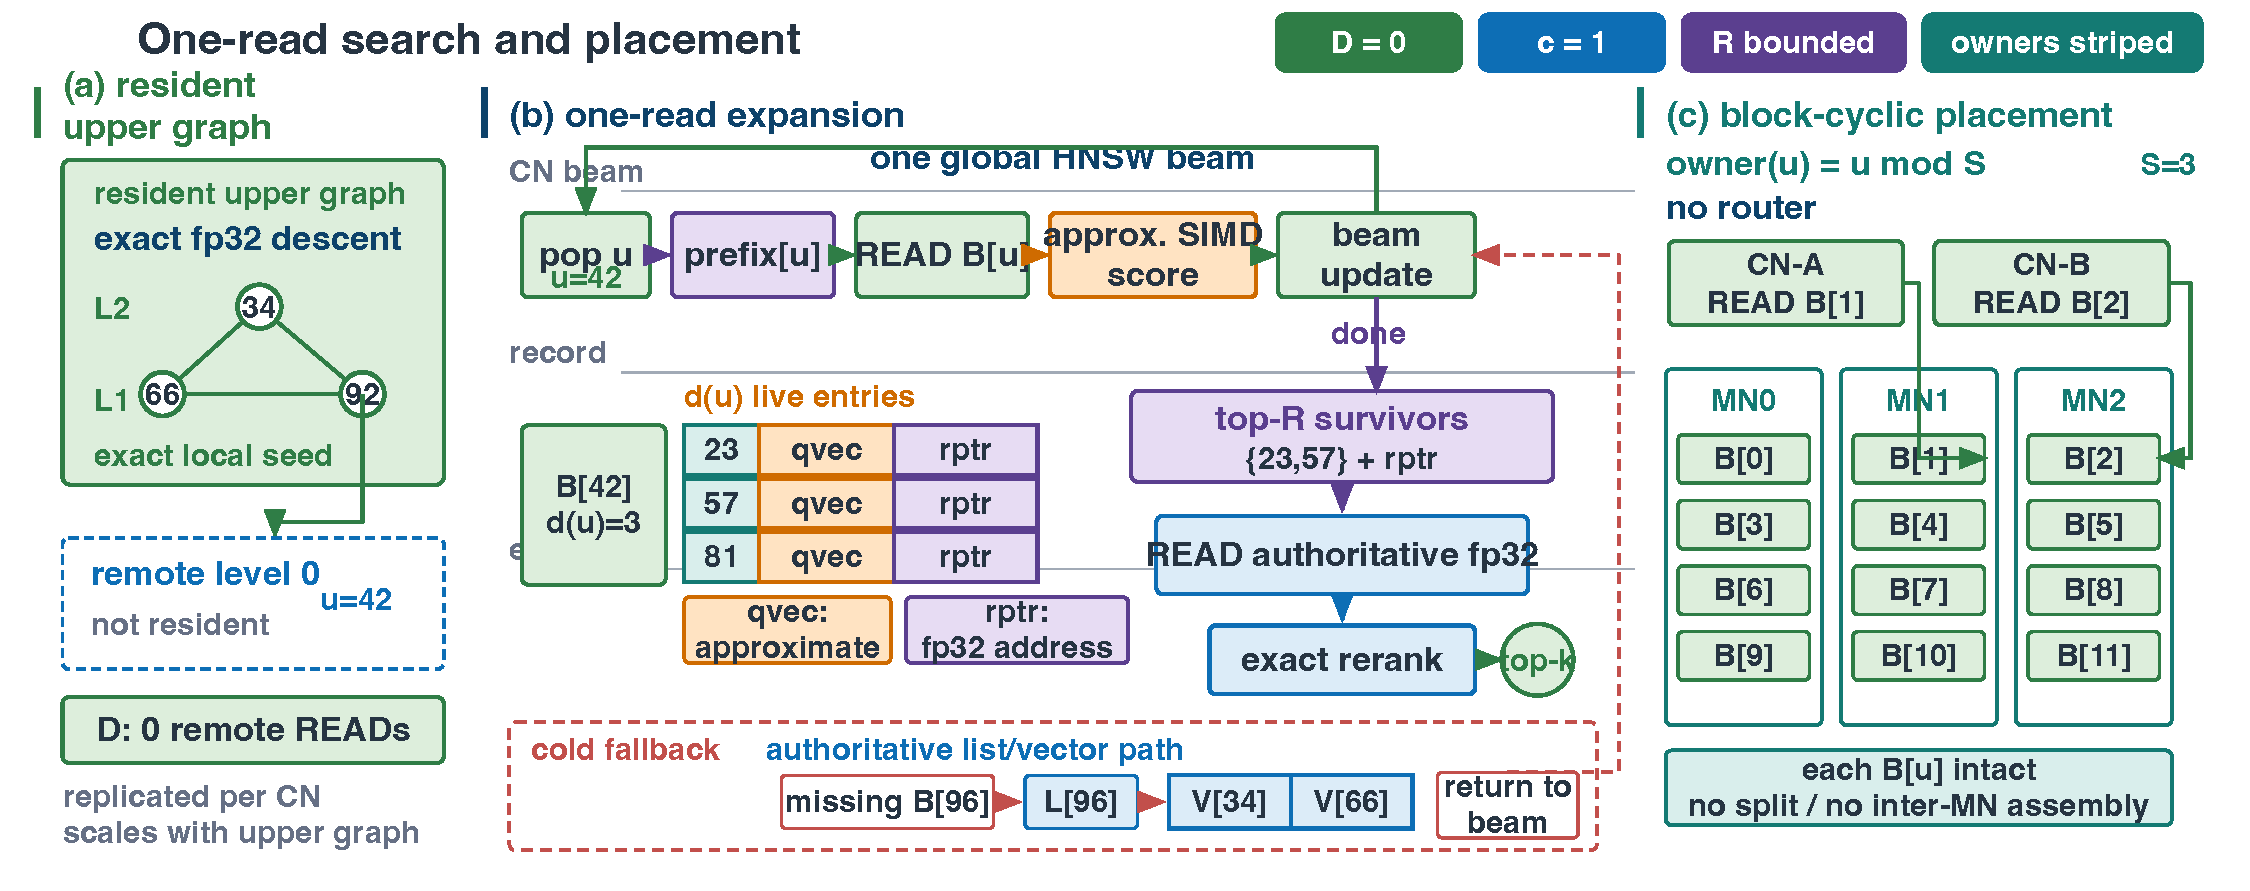
\includegraphics[width=0.86\textwidth]{figs/fig_search_placement.pdf}
\caption{Search and placement: (a) exact resident upper layers remove remote
descent; (b) one $B[u]$ read drives the global beam, with authoritative
fallback and fp32 rerank; (c) block-cyclic ownership places intact records on
passive MNs.  Only compact-code beam scoring is approximate.}
\Description{A resident graph produces the level-0 seed; a CN and RDMA timeline
shows one-read beam expansion, cold fallback, and exact reranking; and a
placement table maps intact records and direct CN reads to three passive MNs.}
\label{fig:search-placement}
\end{figure*}

\subsection{Resident Navigation}
\label{sec:resident-upper-graph}

After Slab records collapse level-0 retrieval, remote upper-layer descent
becomes a residual serial term.  Figure~\ref{fig:search-placement}(a) removes
those remote accesses by placing an
exact upper-graph copy at each CN\@.  The evaluated SIFT-1M copy contains
\ClaimResidentNodes{} nodes and \ClaimResidentBytesMB{}\,MB of fp32 payload, so
local greedy descent obtains the same level-0 seed and eliminates $D_A(q)$.

This is a CN-resident component of the derived physical access structure, not a
learned or query-result cache.  It targets the serial upper-descent term
$D_A(q)$ rather than reusing arbitrary level-0 objects.  The independent
\ef{} on/off sweep in
Figure~\ref{fig:eval-index-cost}(c) reports its QPS effect and verifies zero
remote upper-layer posts at matched recall.  Its replicated cost scales with the number
and fp32 dimension of upper-layer nodes rather than with the materialized
level-0 Slab region.

\subsection{One-Read Walk and Exact Rerank}
\label{sec:search}

Figure~\ref{fig:search-placement}(b) summarizes the ordinary global HNSW
level-0 beam.  Each popped $u$ first consults CN-local address metadata.  A
materialized hit resolves to $B[u]$; a miss takes the authoritative cold path.
One Slab read then returns live IDs, \texttt{nbr\_qvec} codes, and
\texttt{nbr\_rptr} addresses.  The CN applies the usual tests, SIMD-scores the
codes, updates the beam, then fetches fp32 vectors for the bounded top-$R$ to
return exact top-$k$ among those survivors.

Because $R$ grows with search width, one rerank must not overrun a verbs send
queue.  SlabWalk derives a per-coroutine chunk from the shared send-queue
capacity of its RDMA queue pair (QP), groups each chunk by MN, and posts one
work-request (WR) chain with a signaled tail per owner.  The chunks preserve
candidate order while bounding outstanding rerank WRs independently of $R$.

The global graph is unchanged; compact codes alone may perturb beam order
before rerank.  SlabWalk widens the approximate beam and reranks a bounded set,
whose final order is exact if it contains the true top-$k$.  On evaluated L2
datasets, int8-code recall tracks the node/vector baseline across the measured
frontier; TTI exposes the inner-product boundary.  Disabling compact
scoring returns the authoritative node/vector path because there is no
fp32-in-Slab scoring mode.

\subsection{Block-Cyclic Placement}
\label{sec:serving}

Figure~\ref{fig:search-placement}(c) maps each intact $B[u]$ to passive owner
$u\bmod S$ and keeps its local offset in the \texttt{RemotePtr}.  Because each
record remains contiguous, an expansion uses one read without a remote directory,
router, or inter-MN assembly even when bytes shift the bottleneck to one NIC\@.

Block-cyclic ownership stripes record owners; it does not by itself guarantee
equal instantaneous link traffic.  It deliberately gives up cross-record
locality because one hop's bytes already reside in $B[u]$.  Rather than assume
perfect balance, Figure~\ref{fig:eval-index-cost}(f) measures per-MN traffic and
memory directly as the stripe count changes.  The deterministic map lets any CN
compute a record's owner from local metadata; we do not evaluate aggregate
multi-CN scale-out (Section~\ref{sec:eval-index-cost}).

At full materialization and resident descent, the passive-RDMA path approaches
$E_A(q)+R_A(q)$ remote accesses rather than the node/vector path's
$D_A(q)+\sum_u(1+m_A(q,u))+R_A(q)$.  Section~\ref{sec:eval-overall} measures the resulting
post, byte, and throughput changes at the same search settings and reports
recall alongside every point.  Section~\ref{sec:deployment} next describes how
the derived records are built and checked without changing authoritative
ownership.

%================================================================
\section{Construction and Offline Refresh}
\label{sec:deployment}

\begin{figure*}[t]
\centering
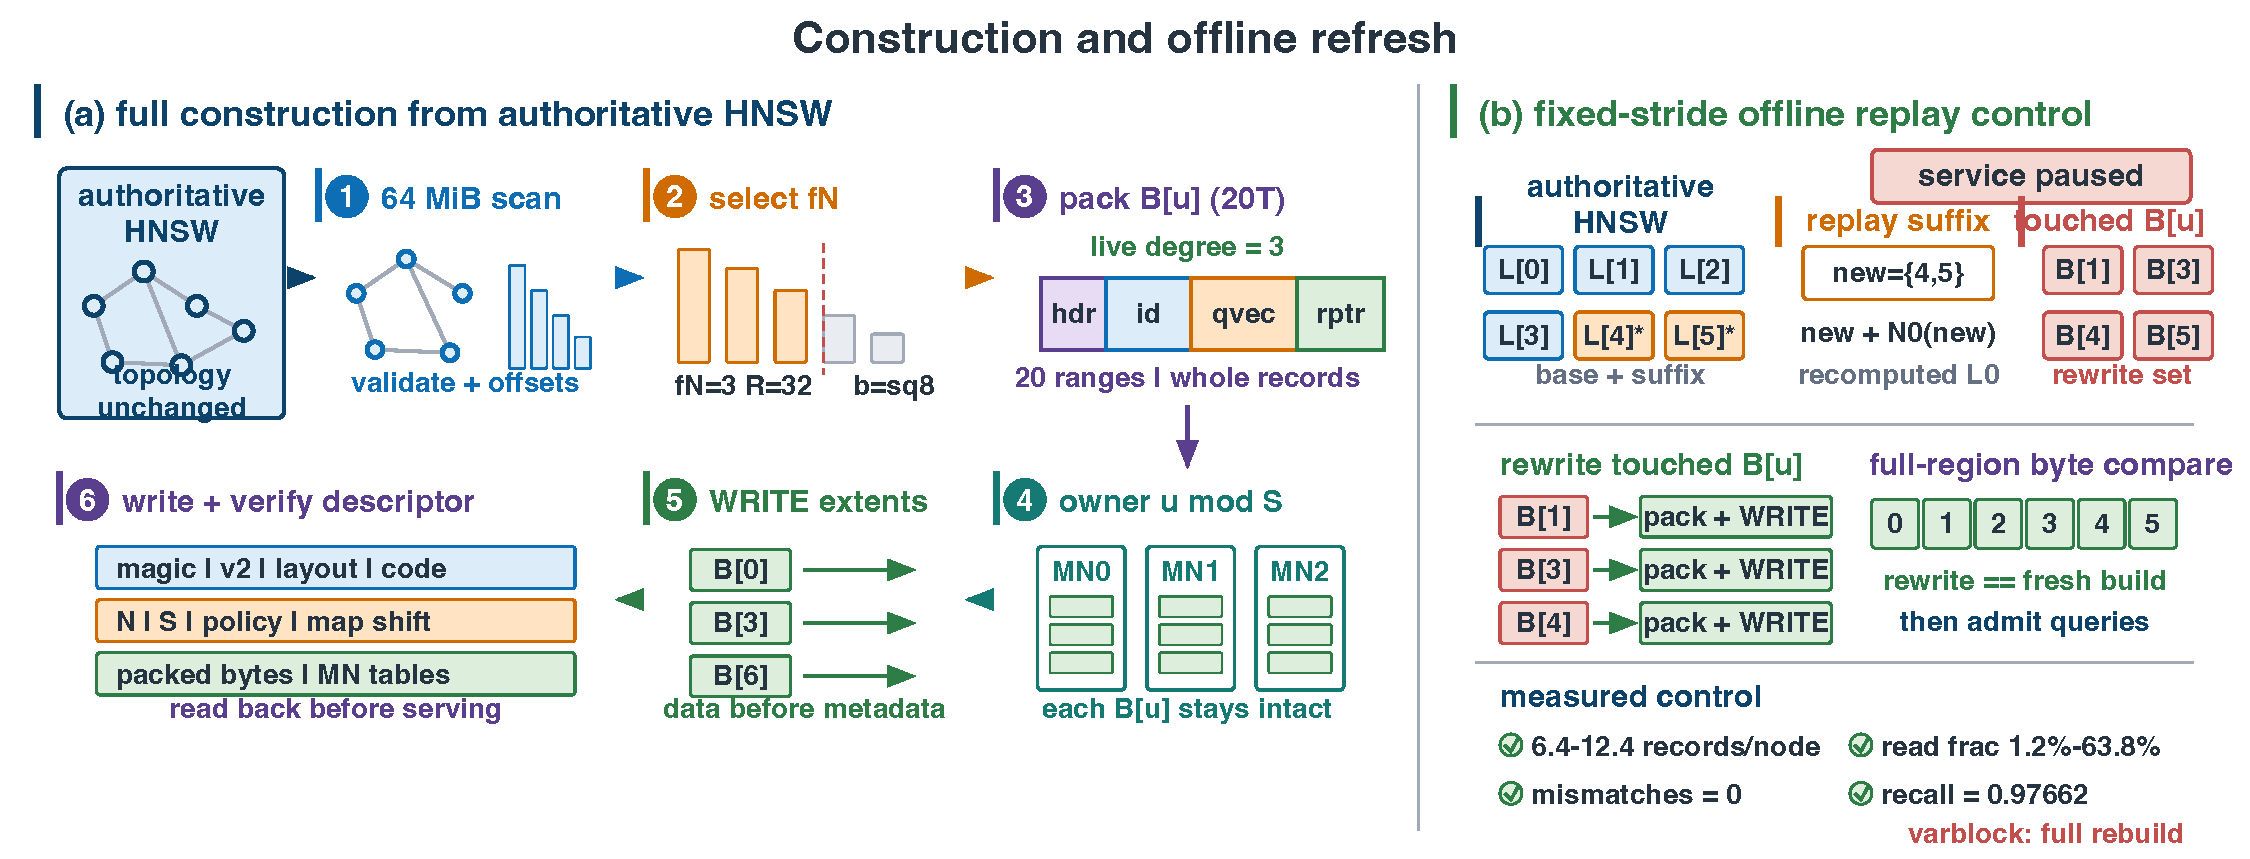
\includegraphics[width=0.86\textwidth]{figs/fig_construction_refresh.pdf}
\caption{Derived-state lifecycle.  (a) Full construction packs and places Slabs,
then writes and verifies the final descriptor.  (b) The fixed-stride offline replay rewrites
records affected by an insertion suffix and compares the result with fresh
materialization.  It measures rewrite amplification, not online refresh.}
\Description{The left state derives, places, and verifies a self-describing
access structure.  The right state replays an insertion suffix while serving
is paused, rewrites touched fixed-stride records, and compares the region with
fresh materialization.}
\label{fig:construction-refresh}
\end{figure*}

\subsection{Full Construction}

Figure~\ref{fig:construction-refresh}(a) starts from a built authoritative
HNSW.  An initiating CN reads and validates records, counts in-degree, and
selects the top-$fN$.  It then encodes live payloads and packs records and
prefixes.  For the full fixed-record construction evaluated in
Section~\ref{sec:eval-rebuild}, pinned workers assemble disjoint UID ranges into
one bounded 64\,MiB registered staging buffer; the CN publishes each contiguous
window with one RDMA WRITE instead of one WRITE per record.  Variable and
budgeted layouts retain record-granular publication.  The builder writes the
descriptor last with the version, layout, code, ownership, and per-MN extent
metadata, reads it back, and verifies it before serving begins.  This ordering
is an offline construction check, not an atomic publication protocol.
Builder memory holds the validated authoritative snapshot.  The builder
hands that same snapshot to resident-upper-graph construction before releasing
it and reuses the deterministic RaBitQ rotation when reconstructing serving
state, avoiding a second authoritative scan and a second rotation build.
Serving CNs validate the descriptor before enabling Slab reads and then copy
the exact upper layers.

The builder never mutates HNSW topology.  Slab bytes form a derived access
structure that can be discarded and rebuilt from the authoritative index.
Section~\ref{sec:eval-rebuild} reports derived-pass wall time, stage
composition, builder peak DRAM, and final bytes separately from HNSW
construction.  A fast derived pass is not evidence of a fast billion-scale
graph build.

\subsection{Offline Refresh Boundary}

Figure~\ref{fig:construction-refresh}(b) shows the narrower refresh path that
we evaluate.  With queries not yet admitted, we replay the final authoritative
graph as a base prefix plus an insertion suffix.  We select the suffix nodes
and their final level-0 neighbors, invalidate those fixed-stride Slab records,
and rewrite them in place with the original quantizer.  A full-region
comparison then checks every byte against fresh materialization.  Across the
evaluated suffixes, the control selects
\ClaimRefreshMinRecords--\ClaimRefreshMaxRecords{} records per suffix node; all
admitted replays are byte-identical to fresh materialization.  Variable records
require full reconstruction because a degree
change can shift later offsets.  This experiment bounds derived-state rewrite
amplification; the implementation does not provide concurrent HNSW mutation,
reader epochs, atomic publication, or crash recovery.

\subsection{Implementation and Passivity}

SlabWalk extends SHINE's RDMA HNSW substrate on the CN side~\cite{shine}.
The same binary independently toggles Slab records, resident navigation,
variable records, and placement.  Exact-copy mechanisms can return to the
authoritative path without changing graph state; disabling compact scoring
returns the node/vector baseline.  MNs only allocate and register regions and
expose their bytes to one-sided reads and writes.  They run no index operator, router,
distance kernel, or deserializer.

%================================================================
\section{Evaluation}
\label{sec:eval}

We ask four questions.  \textbf{Q1:} Does expansion-oriented retrieval improve
the recall--throughput frontier over node/vector and partition-fetch access?
\textbf{Q2:} Does operation cost explain query throughput, and when do
concurrency, incomplete records, or deployment topology move the bottleneck?
\textbf{Q3:} What CN memory, MN storage, and transferred bytes does the physical
design require, and can an offline rule select a measured layout under these
constraints?  \textbf{Q4:} What are the cost and supported semantics of
construction and offline refresh, and where do compact codes lose recall?  We
fix query pools and measurement rules across systems while retaining each
native deployment; Section~\ref{sec:eval-protocol} states the remaining
topology differences.
Figure~\ref{fig:eval-frontier-curves} presents Q1 as one repeated frontier
matrix: seven 1M workloads test breadth and three 10M workloads test scale.

\begin{figure*}[t]
\centering
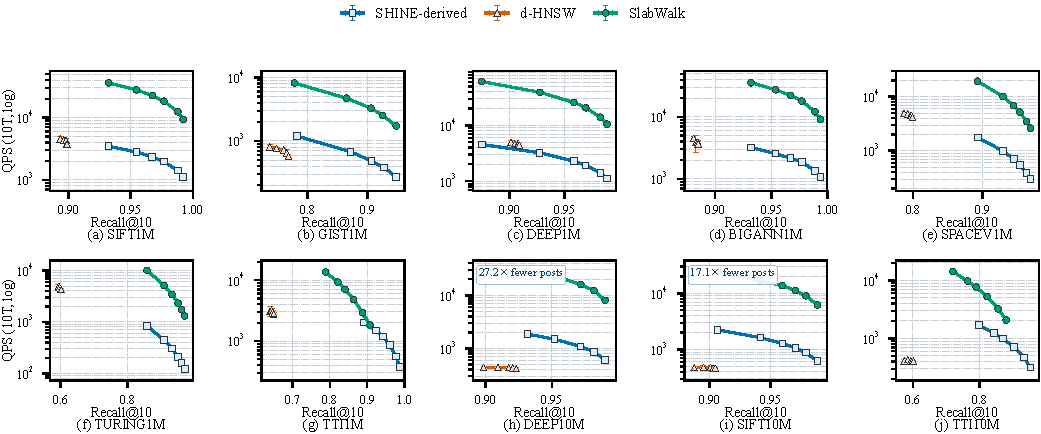
\includegraphics[width=0.94\textwidth]{figs/eval_frontier_curves.pdf}
\vspace{-0.35em}
\caption{Recall@10--QPS frontiers at ten workers.  Panels (a--g) cover seven
1M workloads; panels (h--j) cover DEEP, SIFT, and TTI at 10M.  Every panel
compares the SHINE-derived node/vector path, native d-HNSW, and \sys{}.
Points are five-run means with 95\% Student-$t$ intervals; the DEEP-10M and
SIFT-10M annotations give matched-high-recall reductions in posted reads/query
between the graph-preserving paths.}
\Description{Ten Recall@10--QPS panels compare SHINE-derived, fixed-routing
d-HNSW, and SlabWalk at ten workers.  Seven panels provide 1M workload breadth
and three provide 10M scale evidence.  All points include confidence intervals
from five runs over content-identical 10K query pools; the 10M panels annotate
eligible reductions in posts per query.}
\label{fig:eval-frontier-curves}
\end{figure*}

\subsection{Methodology}
\label{sec:eval-protocol}

\paragraph{Testbed and workloads.}
We use seven 100\,Gbps RoCE\,v2 nodes, each with two 20-core Xeon Gold 5218R
CPUs and a ConnectX-6 DX NIC; nodes 1--3 have 192\,GB DRAM and nodes 4--7
have 128\,GB\@.  The hosts run Ubuntu 20.04, Linux 5.4.0, and 4096-byte active
MTU (NIC firmware 22.27.6106).  \mn{}s are passive
one-sided targets; \cn{}s perform all graph and distance work.  Unless stated
otherwise, runs use eight coroutines per worker, one \mn{}, sq8 scoring codes,
and bounded fp32 rerank $R{=}\max(k,\ef/2)$.  The matched frontier in
Figure~\ref{fig:eval-frontier-curves} uses two coroutines per worker for both
graph-preserving paths; other experiments state their concurrency separately.
The 1M breadth matrix covers SIFT (128D), GIST (960D), DEEP (96D), BIGANN
(128D), SPACEV and TURING (100D each), and TTI (200D).
All use L2 except TTI, which uses inner product.  The scale matrix uses
DEEP-10M, SIFT-10M, and TTI-10M at the same respective dimensions and metrics.
The 1M graphs use $(M,\mathit{efConstruction})=(16,100)$; the 10M graphs use
$(32,200)$ for DEEP and $(16,100)$ for SIFT and TTI\@.  On DEEP-10M, both graph-preserving paths load the same retained
GraphBeyond HNSW dump.  For SIFT and TTI, we build one authoritative graph with
hnswlib 0.8.0~\cite{hnswlib} (seed 47), convert only its serialization, and
validate every vector, level, neighbor ID, pointer, and padding byte after
conversion.  SHINE-derived and \sys{} then load the same dump for each
dataset.  The same topology control holds for each 1M SHINE-derived/\sys{}
pair.  d-HNSW constructs its native partitioned index from the same base
vectors but does not share this HNSW topology.  Mechanism and resource controls
reuse the 1M workloads; GIST's 960-dimensional payload stresses storage and
bandwidth.  We report Recall@10, aggregate QPS, RDMA posts/query, bytes/query,
and latency where the implementation exposes it.

\begin{table}[t]
\centering\scriptsize
\caption{Scale-frontier inputs.  Every dataset has $N{=}10$M and 10K query
rows.  ``GT'' is the retained exact-neighbor depth used to compute Recall@10.}
\label{tab:frontier-inputs}
\setlength{\tabcolsep}{3.2pt}
\begin{tabular}{@{}lrrrr@{}}
\toprule
Dataset & $d$ & Metric & $(M,\mathit{efC})$ & GT \\
\midrule
DEEP-10M & 96 & L2 & $(32,200)$ & 100 \\
SIFT-10M & 128 & L2 & $(16,100)$ & 1000 \\
TTI-10M & 200 & IP & $(16,100)$ & 100 \\
\bottomrule
\end{tabular}
\end{table}

Across physical file formats, canonical content hashes verify that all three
systems consume the same 10K query and ground-truth rows for each of the ten
frontier datasets.  For TTI, an
independent exact inner-product recomputation also verifies top-10 set identity
for query rows 0, 4999, and 9999.

\paragraph{Comparators.}
For the graph-preserving baseline, we disable Slabs, resident navigation, and
the generic cache in the same binary with \texttt{--lavd 0}.  We label this
node/vector path \emph{SHINE-derived}; it is not an official SHINE run.  Cache
and routing variants appear only as separately labeled
controls.  The Slab, resident-navigation, variable-record, and placement gates
share the authoritative graph, queues, kernels, coroutines, RDMA runtime, and
memory registration with that denominator.  This same-binary pairing controls
topology and runtime, but its end-to-end QPS difference still includes compact
scoring and bounded rerank in addition to the changed record.  We run the
released d-HNSW implementation on the same cluster
while preserving its partitioning, serialization, and batch
pipeline~\cite{dhnsw}.  Its released harness co-locates server and client on one
RDMA host; \sys{} uses separate \cn{} and \mn{} hosts.  The frontier therefore
uses d-HNSW as a native-deployment reference on the same hardware pool, not as
a topology-normalized ablation.  It uses ten workers for every system, never
our 40-worker peak.  The released fixed-routing configuration is held constant
while its sub-search \ef{} is swept.  We make two evaluator
compatibility fixes: the released query loop's hard-coded $k{=}1$ now honors
$k{=}10$, permitting set Recall@10; and TTI propagates its Angular/IP metric
through the server and client.  We do not change index construction, routing,
partition fetch, deserialization, or subgraph search.  QPS is recomputed from
the completed per-thread query counts and wall-clock time of the fixed pool.

\paragraph{Measurement protocol.}
The primary frontier, model-control matrix, and query-robustness matrix each
use one warmup followed by five measured runs and report means with two-sided
95\% Student-$t$ intervals.  We retain every completed measured run and apply
no post hoc outlier removal.  At every frontier point, all three systems process
the same 10,000 query and ground-truth rows exactly once at ten workers; a
cross-format content fingerprint checks the graph-path and d-HNSW inputs before a
point can enter the figure.  Other labeled endpoints and breakdowns use
independently repeated medians rather than values copied from a sweep, and state
their repeat count where it differs.  Tail results use separate 10K-query
no-batching traces.  The exact-byte advisor study uses one separately sealed
builder-policy binary for all 162 rows because byte admission was implemented
after the query-frontier freeze.  Its policies are compared only within that
campaign; none of its absolute QPS values enters the system frontier.
Construction uses five independent derived-build runs with
20 builder threads and one post-build query worker, and reports the mean with a
two-sided 95\% Student-$t$ interval.
For each 10M headline annotation, the evidence gate selects the highest
same-$\ef$ pair where both graph-preserving paths reach at least
\ClaimFrontierRecallFloor{} recall and differ by at most
\ClaimFrontierRecallTolerance{}.

\subsection{Q1: End-to-End Frontier}
\label{sec:eval-overall}

Figure~\ref{fig:eval-frontier-curves} contains one controlled same-binary
comparison and one native-deployment comparison.  Only the first supports a
causal interpretation: SHINE-derived and \sys{} share the HNSW
topology, search width, workers, query pool, queues, and runtime.  Their
posts/query contrast directly measures access amplification; their QPS contrast
includes expansion records, compact scoring, resident descent, and bounded
rerank.  We therefore compare complete recall--QPS curves instead of treating a
common \ef{} as equal quality.  The released fixed-routing
d-HNSW reference retains its meta-HNSW and partition path, so it measures a
different coverage/transfer tradeoff, not an ablation of the same walk.
At the eligible matched-high-recall DEEP-10M and SIFT-10M pairs, \sys{}
delivers \ClaimFrontierQpsMin--\ClaimFrontierQpsMax$\times$ the QPS
while issuing \ClaimFrontierPostsMin--\ClaimFrontierPostsMax$\times$ fewer
posted reads than the SHINE-derived path.  The completeness control in
Section~\ref{sec:eval-scaling} isolates the access-unit effect; the cache control
in Figure~\ref{fig:physical-units} shows why reuse alone is insufficient.

The seven 1M panels in Fig.~\ref{fig:eval-frontier-curves} span dimensions,
source representations, and both L2 and inner-product search.  The three 10M
panels repeat the comparison after a tenfold increase in index cardinality, so
the result is not reported from a single dataset or selected operating point.
On the three 10M scale
panels, under the evaluated release configuration, d-HNSW's
best observed Recall@10 is \ClaimDhnswDeepRecall{} on DEEP,
\ClaimDhnswSiftRecall{} on SIFT, and \ClaimDhnswTtiRecall{} on TTI\@.
Increasing sub-search \ef{} cannot recover candidates outside the partitions
selected by the fixed meta-search and routing fan-out.  These are measured
configuration boundaries, not intrinsic ceilings for every partition design.
TTI also separates access efficiency from representation quality: the current
compact-code SlabWalk configuration reaches a lower recall boundary despite
reducing remote accesses.  Section~\ref{sec:eval-scope} measures the associated
recall--bytes tradeoff; because no fp32-in-Slab path exists, it does not assign
the entire difference to compression alone.

\subsection{Q2: Access Cost and Scaling}
\label{sec:eval-scaling}

\begin{figure*}[t]
\centering
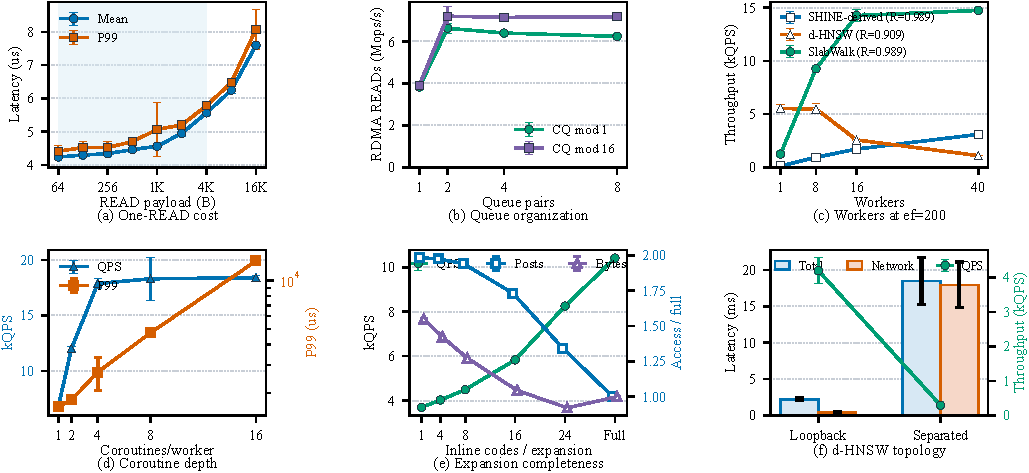
\includegraphics[width=0.84\textwidth]{figs/eval_access_scaling.pdf}
\vspace{-0.35em}
\caption{Access-cost controls: (a) one-READ mean/P99 by payload;
(b) 256-byte READ rate by QP/CQ configuration; (c) three-system worker scaling
at $\ef{=}200$, with observed Recall@10 in the legend; (d) \sys{} coroutine
depth; (e) in-record code count; and (f) d-HNSW topology sensitivity.  Query
panels use DEEP-1M; points show five-run means and 95\% Student-$t$ intervals.}
\Description{Six panels validate the fixed cost of one RDMA read and show
three-system worker scaling, SlabWalk concurrency and expansion-completeness
controls, and d-HNSW topology sensitivity.}
\label{fig:eval-scaling-ablation}
\end{figure*}

The controlled experiment below the ANN stack first checks that the fixed
per-operation premise represented by $\tau$ is not an artifact of the search
implementation.  Across five repetitions, increasing
one-sided READ payload from 64\,B to 4\,KB changes mean latency from
\ClaimRdmaPayloadSmallMeanUs{} to \ClaimRdmaPayloadLargeMeanUs{}\,$\mu$s and
P99 from \ClaimRdmaPayloadSmallTailUs{} to
\ClaimRdmaPayloadLargeTailUs{}\,$\mu$s.  Mean and P99 grow only
\ClaimRdmaPayloadMeanSpan$\times$ and
\ClaimRdmaPayloadTailSpan$\times$, respectively, for a 64$\times$ payload
increase.  At 256\,B, one QP with CQ moderation 1 sustains
\ClaimRdmaQpOneMops\,M READs/s; two QPs with moderation 16 reach
\ClaimRdmaQpTwoMops\,M READs/s.  Changing MTU from 1024 to 4096 changes mean
latency by \ClaimRdmaMtuMeanSpan$\times$, and the two same-node NUMA
placements differ by \ClaimRdmaNumaDiffPct\%.  Outstanding reads raise
one-QP rate from \ClaimRdmaOutsOneMops{} to
\ClaimRdmaOutsSixteenMops\,Mops/s.  Queue organization therefore
moves the service ceiling, but it does not remove the cost paid by each small
READ.

The query path also has a concurrency limit.
Figure~\ref{fig:eval-scaling-ablation}(c) compares scaling shape at the same
$\ef{=}200$ setting and reports each method's observed recall in the legend;
because those recalls differ, we do not present its QPS as a matched-recall
ranking.  In this common-protocol campaign, increasing \sys{} workers from 1
to 40 raises throughput from \ClaimWorkerOneKqps{} to
\ClaimWorkerFortyKqps{}\,kQPS ($\ClaimWorkerGain\times$).  Recall@10 averages
\ClaimWorkerRecall{} across the four worker counts.  A separate
one-factor-at-a-time \sys{} control fixes ten
workers: increasing coroutines from one to four raises throughput from
\ClaimCoroOneKqps{} to \ClaimCoroFourKqps\,kQPS\@.  Raising coroutine depth
from four to sixteen adds only \ClaimCoroFourToSixteenGainPct\% throughput but
raises P99 from \ClaimCoroFourTailMs{} to
\ClaimCoroSixteenTailMs\,ms.  More in-flight work can hide service time; after
the queues saturate, it mainly accumulates waiting time.

The released d-HNSW protocol places client and server on one host, which is
favorable to its routed-partition path.  We retain that protocol for the main
frontier.  As a sensitivity control, we separate the same client and server.
Recall@10 remains \ClaimTopologyRecall{}, while throughput changes from
\ClaimTopologyLoopbackKqps{} to \ClaimTopologyRemoteKqps\,kQPS and mean
latency changes from \ClaimTopologyLoopbackLatencyMs{} to
\ClaimTopologyRemoteLatencyMs\,ms.  The network phase accounts for
\ClaimTopologyRemoteNetworkMs\,ms of the latter.
Figure~\ref{fig:eval-scaling-ablation}(f)
therefore bounds deployment sensitivity rather than replacing the released
configuration in the primary comparison.

Result width and query skew do not create another remote-access path.
Across $k{=}1$--100, throughput varies by \ClaimTopKQpsSpanPct\%, while posts/query and
bytes/query are unchanged; scoring the expansion, rather than returning the
final list, dominates remote work.  Zipf-1.0 queries differ from uniform by
\ClaimZipfQpsDiffPct\% in throughput and \ClaimZipfTailDiffPct\% in P99.
Timing-enabled and timing-disabled runs
have overlapping 95\% intervals; within this experiment, instrumentation does
not produce a resolved throughput difference.

A direct completeness control varies how many of a 32-neighbor expansion's
scoring codes remain in the first Slab read.  With only one code inline, the
walk attains Recall@10 \ClaimColocationRecall{} but, relative to a complete
record, loses \ClaimColocationQpsLoss\% QPS while issuing
\ClaimColocationPostIncrease\% more posts and transferring
\ClaimColocationByteIncrease\% more bytes.  Returning an incomplete expansion
therefore recreates the access amplification that the physical record is
meant to remove; contiguity alone is insufficient.

The completeness control and post counter rule out a layout-only CPU
explanation.  The evaluated \sys{} configuration changes the remote object,
scoring representation, and rerank path together.  Its post counter verifies
the reduction from $c_A(q,u)=1+m_A(q,u)$ toward one posted READ per Slab-backed
expansion; Figure~\ref{fig:eval-frontier-curves} supplies the quality-aware
three-system comparison.  Because the implementation has no fp32-in-Slab mode,
we do not attribute the headline QPS factor to record layout alone.

\subsection{Q3: Index Cost and Deployment}
\label{sec:eval-index-cost}

\begin{figure*}[t]
\centering
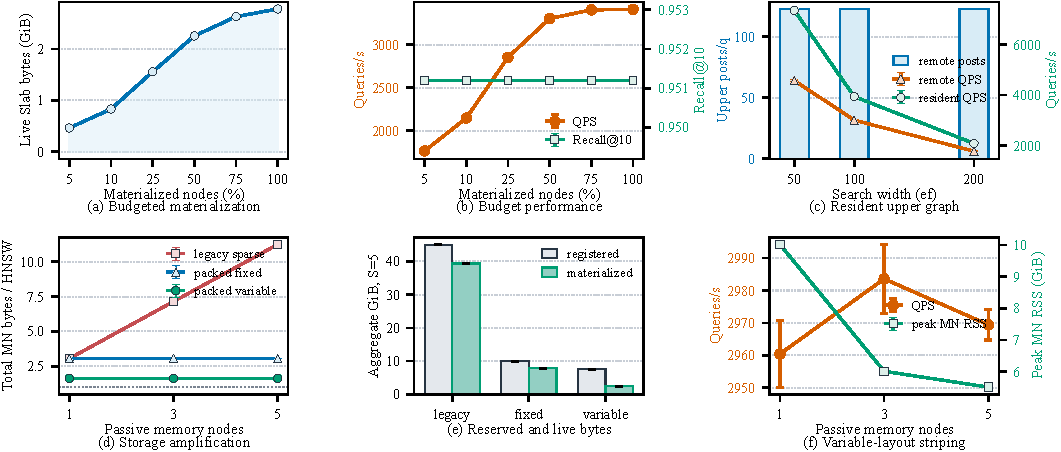
\includegraphics[width=0.84\textwidth]{figs/eval_index_cost.pdf}
\vspace{-0.35em}
\caption{Physical-design costs.  GIST-200K: (a--b) materialization bytes,
QPS, and recall.  SIFT-1M: (c) resident upper navigation.  GIST-1M: (d--f)
storage amplification, reserved versus live bytes, and packed-variable QPS
and peak per-MN RSS under striping.  Points show five-run means and 95\%
Student-$t$ intervals.}
\Description{Six panels show the byte and query effects of bounded
materialization, resident upper navigation, packed layouts, and block-cyclic
placement.}
\label{fig:eval-index-cost}
\end{figure*}

\paragraph{Materialization budget ($\mathcal{M}$).}
Figure~\ref{fig:eval-index-cost}(a,b) treats the budget as a measured physical
choice rather than a free parameter.  On GIST-200K, the 5\% and full policies
materialize \ClaimBudgetFiveGiB{} and \ClaimBudgetFullGiB{}\,GiB, respectively;
the companion panel reports QPS and recall for every feasible point.  A
deployment with fixed MN memory and recall targets can therefore reject
infeasible points, then rank the retained policies.  We evaluate that rule on
sealed SIFT-1M, DEEP-1M, and GIST-1M sweeps at 512\,MiB, 1\,GiB, and 2\,GiB.
The advisor sees repeats 0--2 and is evaluated once on repeats 3--5.  Across
\ClaimAdvisorCellCount{} dataset--budget cells it selects the access-benefit
policy in \ClaimAdvisorBenefitCells{} and in-degree in
\ClaimAdvisorIndegCells{}; held-out QPS is at least
\ClaimAdvisorMinPercent\% of the feasible per-cell oracle, with a
\ClaimAdvisorGeoPercent\% geometric mean.  This is a strict post-hoc split of a
pre-existing campaign, not prospective prediction or online optimization.

\paragraph{Resident upper graph ($D$).}
Figure~\ref{fig:eval-index-cost}(c) toggles only exact upper navigation.  At
three search widths, it reports remote upper posts and the corresponding QPS
while recall remains identical.  At \ef{=}100, the remote path spends
\ClaimResidentRemotePosts{} posts/query on upper navigation; residency removes
those posts and raises QPS by \ClaimResidentQpsGain\%.  The copy contains
\ClaimResidentNodes{} SIFT nodes and \ClaimResidentBytesMB{}\,MB of fp32 payload
per CN.  It is replicated per CN, so we account for this state separately from
striped MN bytes.

\paragraph{Record layout and striping ($\mathcal{M},B$).}
Figure~\ref{fig:eval-index-cost}(d,e) compares legacy sparse, packed fixed, and
live-prefix records on GIST-1M.  At five MNs, their storage amplifications are
\ClaimLegacyAmplification$\times$, \ClaimFixedAmplification$\times$, and
\ClaimVariableAmplification$\times$.  The variable layout materializes
\ClaimVariableSidecarGiB{}\,GiB and reaches \ClaimVariableCnRssGiB{}\,GiB CN
peak RSS.  We compute each ratio from the authoritative HNSW extent consumed by
the builder and report registered capacity separately from materialized bytes.
Variable addressing contributes $8(N+S)$ bytes per CN; partial materialization
adds a $4N$-byte budget map.  Process RSS additionally includes graph, query,
and allocator state.

Holding the packed-variable layout fixed, panel (f) changes only the number of
MN targets.  From one to five MNs, QPS changes from
\ClaimVariableOneMnQps{} to \ClaimVariableFiveMnQps{}, while peak per-MN RSS
falls from \ClaimVariableOneMnRssGiB{} to
\ClaimVariableFiveMnRssGiB{}\,GiB and read-byte Gini remains at most
\ClaimVariableReadGini.  Under the shared-NIC testbed, striping therefore
distributes capacity and passive-memory load; it is not a claim of throughput
scale-out.  It requires neither a query router nor a different graph walk.

\subsection{Q4: Construction, Offline Refresh, and Boundaries}
\label{sec:eval-rebuild}
\label{sec:eval-scope}

Figure~\ref{fig:eval-boundary}(a--c) isolates the cost of deriving Slabs after
loading the authoritative HNSW\@.  All runs use full, fixed-record
materialization and 20 builder threads; SIFT and DEEP use sq8, while GIST uses
RaBitQ-2.  Mean times
are $\ClaimBuildOneMSiftSeconds\pm\ClaimBuildOneMSiftCiSeconds$,
$\ClaimBuildOneMDeepSeconds\pm\ClaimBuildOneMDeepCiSeconds$, and
$\ClaimBuildOneMGistSeconds\pm\ClaimBuildOneMGistCiSeconds$ seconds for SIFT,
DEEP, and GIST (95\% Student-$t$ CIs).  Median stage shares show that record
materialization dominates SIFT and DEEP, whereas GIST divides its build time
among fetching/parsing, code generation, and record materialization.  Mean
peak builder RSS is \ClaimBuildOneMSiftRssGiB{},
\ClaimBuildOneMDeepRssGiB{}, and
\ClaimBuildOneMGistRssGiB{}\,GiB; final Slab structures are
\ClaimBuildOneMSiftRegionGiB{}, \ClaimBuildOneMDeepRegionGiB{}, and
\ClaimBuildOneMGistRegionGiB{}\,GiB.  These are added access-structure costs,
not HNSW build time.

The 10M campaign measures the same derived-build boundary rather than
extrapolating from 1M.  The complete derived Slab build takes
$\ClaimBuildTenMDeepSeconds\pm\ClaimBuildTenMDeepCiSeconds$,
$\ClaimBuildTenMSiftSeconds\pm\ClaimBuildTenMSiftCiSeconds$, and
$\ClaimBuildTenMTtiSeconds\pm\ClaimBuildTenMTtiCiSeconds$ seconds for DEEP,
SIFT, and TTI; resident-upper construction takes
\ClaimBuildTenMDeepResidentSeconds{}, \ClaimBuildTenMSiftResidentSeconds{}, and
\ClaimBuildTenMTtiResidentSeconds{} seconds.  Their materialized structures
occupy \ClaimBuildTenMDeepGiB{}, \ClaimBuildTenMSiftGiB{}, and
\ClaimBuildTenMTtiGiB{}\,GiB.  Each value is the mean of five independent
runs, and each reported Slab-build interval is a two-sided 95\% Student-$t$
interval.

Figure~\ref{fig:eval-boundary}(d--e) evaluates the fixed-stride offline replay
control.  Replayed
suffixes of 1K--100K select $\ClaimRefreshMinRecords$--$\ClaimRefreshMaxRecords$
records per suffix node; after a
one-time CN mirror, subsequent replays fetch only the selected authoritative
records.  Invalidating and rewriting those records yields zero mismatches
against fresh full-region materialization, and the subsequent query run retains
recall \ClaimRefreshRecall{}.  These rows quantify selection and rewrite amplification under
paused serving; they do not demonstrate live insertion, reader isolation, or
failure recovery.

Figure~\ref{fig:eval-boundary}(f) bounds the code claim on TTI\@.  Sq8 and
RaBitQ-2/4 reduce the remote payload but reach
\ClaimTtiSqEightRecall{}/\ClaimTtiRqTwoRecall{}/\ClaimTtiRqFourRecall{} recall.
The authoritative fp32 node/vector path reaches \ClaimTtiFpRecall{} recall and
\ClaimTtiFpQps{} QPS\@.  It uses \ClaimTtiFpPosts{} posts/query and a
substantially larger payload.  Since there is no
fp32-in-\xblock{} path, these points show the recall boundary of the current
compact-code SlabWalk configuration; they do not isolate compression as the
only cause.

Queue-safe rerank chunking bounds outstanding WRs but does not remove the
exact-read work of a wider $R$.  Additional \mn{}s distribute storage and load,
but cannot add throughput once bytes reach the shared link.  The controls mark
where posted-operation reduction stops determining the operating point; they
do not imply that one layout dominates every metric.

\begin{figure*}[t]
\centering
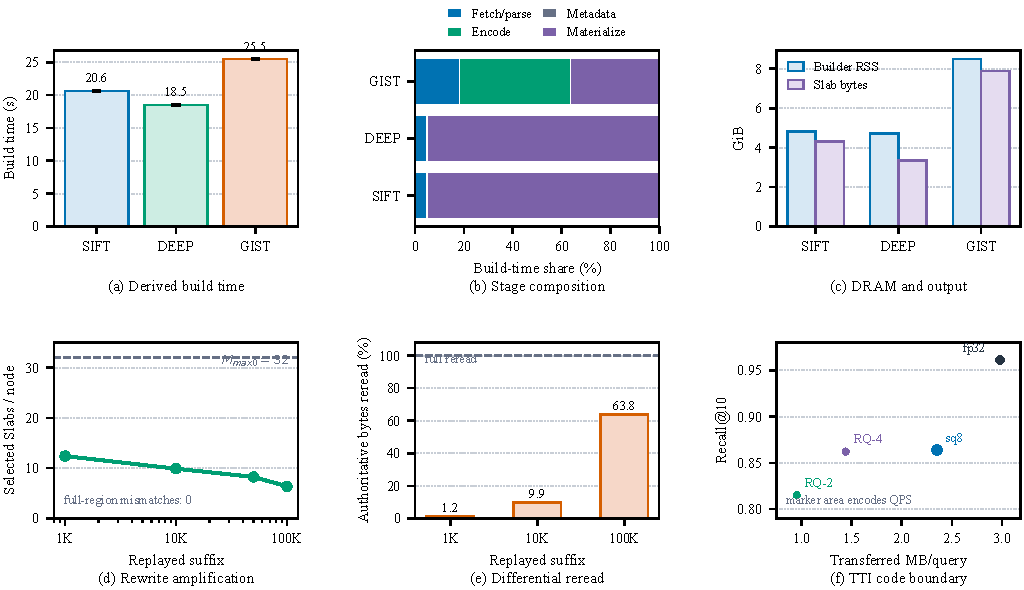
\includegraphics[width=0.84\textwidth]{figs/eval_lifecycle_boundaries.pdf}
\caption{Lifecycle and boundaries: (a--c) Slab build time, stages, DRAM, and
bytes ($n{=}5$); (d--e) fixed-stride offline replay, showing selected records
and authoritative bytes reread; and (f) TTI recall--bytes tradeoff, with
marker area encoding one-worker QPS\@.  Replay and TTI points are single-run
scope controls; every retained source is hash-linked to the plotted CSV.}
\Description{Six panels show repeated Slab build time, build-stage shares,
builder memory and output bytes, offline record rewrite/read amplification,
and the TTI compact-code boundary.}
\label{fig:eval-boundary}
\end{figure*}

%================================================================
\section{Discussion}
\label{sec:discussion}

\textbf{Selecting a deployment point.}
SlabWalk exposes a physical design space rather than one universal setting.
An operator begins with an authoritative HNSW, a recall target, and CN and MN
memory limits.  Code and record format are chosen for the metric and dimension;
the materialization fraction $f$ is then swept under the MN budget.  For each
retained point, $\ef$ and $R$ determine the recall--throughput operating range.
Points that violate recall, resident-memory, Slab-byte, or link constraints in
Eq.~\ref{eq:deployment-constraints} are discarded.  The offline advisor then
ranks only the retained measured candidates by the lower 95\% QPS bound.  The
GIST budget sweep in Figure~\ref{fig:eval-index-cost}(a,b) is one instance of
this process:
early records remove many accesses, whereas later records consume storage for
smaller throughput gains.  Increasing $S$ addresses per-MN capacity and load;
under a shared NIC it should not be interpreted as a throughput setting.  The
chosen tuple $(f,b,S,R)$ and its layout metadata are stored in the descriptor,
so serving CNs do not infer physical policy at query time.

\textbf{When an expansion is the right object.}
The expansion unit is specific to a passive, global-graph HNSW walk.  It is
appropriate when the next candidate cannot be chosen until the current
neighbor IDs and scoring payloads arrive, and those dependencies fit in one
bounded record.  Node/vector retrieval remains reasonable when fine-grained
remote loads are cheap enough or reuse is high enough to amortize their access
path.  A routed partition can be preferable when routing sharply limits the
searched subgraphs and partition transfer and deserialization amortize over
enough useful local work.  SlabWalk occupies neither endpoint: it preserves
the global HNSW walk but changes the stored object returned by one access.
Figure~\ref{fig:physical-units} and Table~\ref{tab:remote-objects} make these
operator and state differences explicit; the evaluation does not claim that
one organization dominates every workload or hardware interface.

\textbf{The next limiting resource.}
Reducing $\Omega$ does not remove the other terms in
$\mathcal{K}_A=\langle\Omega,\mathcal{B},U,\mathcal{S}\rangle$.  Once posted
operations cease to bind, compact-code quality, rerank reads, CN scoring, or
link bytes can determine the operating point.  The GIST results expose the
storage cost of high-dimensional payloads, and TTI exposes a representation
boundary: the evaluated compact codes save bytes but do not match the fp32
node/vector recall.  A larger $R$ can recover more survivors only by adding
authoritative reads, while additional MNs cannot bypass a shared link.  These
are not secondary implementation details; they are the resource consequences
of materializing more work per remote object.

\textbf{Ownership and maintenance.}
Slabs are disposable derived state.  The authoritative HNSW owns topology and
fp32 vectors, which permits cold fallback and complete rematerialization.  The
evaluated construction path verifies a descriptor before admitting queries,
and the replay control rewrites fixed-stride records only while service is
paused.  It does not establish concurrent insertion, reader isolation, atomic
version switching, or failure recovery.  Multi-CN deployment has a similarly
clear boundary: each CN replicates the resident upper graph and address tables,
while all CNs can compute a Slab owner from the descriptor.  Our experiments
measure one issuing CN and passive-MN striping; they do not establish aggregate
multi-CN throughput scaling.  Online maintenance and coordinated version
admission remain separate database responsibilities.

%================================================================
\section{Related Work}
\label{sec:related}

\textbf{Page and block units.}
HNSW, NSG, and related graphs preserve adaptive local navigation in
memory~\cite{hnsw,nsg,wangsurvey}.  Disk-resident systems reorganize that work
around the storage page.  DiskANN and SPANN combine graph or posting-list
navigation with compressed payloads~\cite{diskann,spann}; Starling reorders
vertices and searches blocks to increase useful graph work per I/O~\cite{starling};
SSD-optimized pgvector exploits device parallelism and page-level
prefetching~\cite{ssdpgvector}.  These systems establish the medium-specific
physical-design principle that SlabWalk follows.  Their expensive unit is a
page or block; ours is a posted remote operation.

\textbf{Node, expansion, and partition units.}
Vector-search systems commonly shard collections and query per-shard
indexes~\cite{milvus,manu,faiss,faissgpu}.  Disaggregated systems choose a
second physical boundary.  SHINE retains node/vector retrieval while adding
caching, segmentation, and routing~\cite{shine}.  CoTra and DistVS combine
partitioning, collaboration, precision staging, and batched
communication~\cite{cotra,distvs}.  d-HNSW routes to and fetches serialized
sub-HNSW partitions~\cite{dhnsw}; CXL-ANNS uses coherent pooled memory,
prefetching, and near-memory parallelism~\cite{cxlanns}.  SlabWalk materializes
the intermediate unit: one dependency-complete expansion record for a passive
global-graph walk.  It changes the physical record returned by one access,
rather than only its reuse policy or the coverage of a routed subgraph.

\textbf{Database ownership and maintenance.}
Milvus, Manu, and HAKES address collection ownership, distribution, updates,
and multi-stage search~\cite{milvus,manu,hakes}.  ACORN co-designs graph
construction and traversal with filters~\cite{acorn}; NaviX integrates an HNSW
operator into graph-DBMS storage and query processing~\cite{navix}.
GaussDB-Vector and Azure Cosmos DB integrate vector indexes with persistent
records, partitioning, updates, and database availability
~\cite{gaussdbvector,cosmosvector}.  FreshDiskANN and SPFresh support dynamic
index maintenance~\cite{freshdiskann,spfresh}.  SlabWalk contributes a lower
layer that complements these responsibilities: a derived physical access
structure for remote HNSW retrieval.  Its current refresh is offline; it does
not replace transactional index maintenance.  Resident navigation follows a
broader disaggregated-index pattern in which compact CN state guides access to
remote records~\cite{xstore,rolex,sherman,chime,dex}.

%================================================================
\section{Conclusion}
\label{sec:conclusion}

SlabWalk reorganizes a remote HNSW around expansions rather than in-memory node
records or routed subgraphs.  One Slab read supplies the dependencies of one
level-0 graph decision; resident navigation and budgeted layout account for the
serial, storage, transfer, and representation costs that follow.  Across the
evaluated frontiers, this expansion-oriented path reduces access amplification
at matched high recall.  The same experiments expose its limits: compact-code quality,
rerank reads, and offline refresh.  The physical-design rule is to make one
paid remote access return one dependency-complete graph step, then measure the
resource that becomes limiting.

\FloatBarrier
\begin{acks}
OpenAI Codex and ChatGPT were used for code-review support, experiment
orchestration, plotting, and language editing.  The author chose the
experimental design, verified every measurement and citation, and accepts
responsibility for the manuscript.
\end{acks}

\bibliographystyle{ACM-Reference-Format}
\bibliography{refs}

\end{document}
